%  $Description: Author guidelines and sample document in LaTeX 2.09$
%
%  $Author: ienne $
%  $Date: 1995/09/15 15:20:59 $
%  $Revision: 1.4 $
%
%\documentclass[times, 10pt,twocolumn]{article}
\documentclass[conference,final]{IEEEtran}
\usepackage{latex8}
\usepackage{times}

% Users' option
\usepackage{amssymb}
\usepackage{amsmath}
\usepackage{graphicx}
\usepackage{epstopdf}
\usepackage{color}
\topmargin=0.001in
\usepackage{multirow}
\usepackage{booktabs}
\newif\ifdraft
\drafttrue

\renewcommand{\multirowsetup}{\centering}
\renewcommand{\arraystretch}{1.2}
\def\nyc{\centering}

\ifdraft
\newcommand{\fixme}[1]{ { \bf{ ***FIXME: #1 }} }
\newcommand{\jhanote}[1]{ {\textcolor{red} { ***Jha: #1 }}}
\newcommand{\Nkimnote}[1]{ {\textcolor{green} { ***Nkim: #1 }}}
\newcommand{\skonote}[1]{ {\textcolor{blue} { ***Jeff: #1 }}}
\newcommand{\athotanote}[1]{ {\textcolor{green} { ***athota: #1 }}}
\newcommand{\Jkimnote}[1]{ {\textcolor{red} { ***Jkim: #1 }}}
\newcommand{\yyenote}[1]{ {\textcolor{blue} { ***yye00: #1 }}}
\else
\newcommand{\jhanote}[1]{}
\newcommand{\Nkimnote}[1]{}
\newcommand{\fixme}[1]{}
\newcommand{\skonote}[1]{}
\newcommand{\Jkimnote}[1]{}
\fi
% End of users' option

%\documentstyle[times,art10,twocolumn,latex8]{article}

%-------------------------------------------------------------------------
% take the % away on next line to produce the final camera-ready version
\pagestyle{empty}

\newcommand{\up}{\vspace*{-1em}}
\newcommand{\upp}{\vspace*{-0.5em}}
\newcommand{\ts}{$T_{s}$}


%-------------------------------------------------------------------------
\title{Accurate and Efficient Multi-scale Flow Simulation by A Hybrid CFD-MD Approach with Its Runtime Environment}

\author{
 ~\\[-2em]
 Soon-Heum Ko$^{1}$, Nayong Kim$^{1}$, Abhinav Thota$^{1,2}$ (?), \\
 Dimitris Nikitopoulos$^{3}$, Dorel Moldovan$^{3}$ (?), Shantenu Jha$^{*1,2}$\\
 \small{\emph{$^{1}$Center for Computation \& Technology, Louisiana State University, USA}}\\
 \small{\emph{$^{2}$Department of Computer Science, Louisiana State University, USA}}\\
 \small{\emph{$^{3}$Department of Mechanical Engineering, Louisiana State University, USA}}\\
 \small{\emph{$^{*}$Contact Author}}\\
}

%\thispagestyle{empty}

\begin{document}


\maketitle

\begin{abstract}
----- Abstracts from two papers are dragged here. Needs merging later. -----
(From ECCOMAS) Hybrid continuum fluid dynamics (CFD) molecular dynamics (MD) simulation methodology is a reliable simulation approach capable of accurately describing the flow at both molecular and macroscopic scales. In this approach the continuum and molecular domains are coupled through an overlap region that facilitates the exchange of information between them forcing the two descriptions to match each other by imposing constrained molecular dynamics and boundary conditions based on time and spatial averaging of relevant physical properties in the overlap region. Despite the recent developments reported in literature, most of them tested against small idealized pure atomistic simulations, there are a few methodological and implementation issues that need further refinement, testing and validation. Specifically, two sets of issues need further clarification: (1) identify the limits and the optimal conditions for a hybrid implementation (e.g., size of the overlap region, sampling time for atomistic averaging, etc.), (2) asses the feasibility of applying the hybrid approach to unsteady flow problems. Using a hybrid CFD-MD implementation we address these issues by focusing on two classical flow problems: the steady Couette flow and the unsteady Stokes boundary layer flow. An in-house incompressible Navier-Stokes CFD code and the LAMMPS MD package are used as baseline codes in our hybrid scheme. We begin by presenting the results of the stationary flow simulation using MD package, which give us the profile of the velocity field in the atomistic domain. The appropriate hybrid condition acquired from this data is used for the calibration of the hybrid simulations. We validated our hybrid solution package by solving Couette flow and the Stokes boundary layer flow. The results of the Couette flow simulation demonstrate that our implementation accurately describes steady flow profile. The unsteady simulations indicate the presence of a time-lagging in hybrid boundary, which can be viewed as an inherent characteristic of the synchronous coupling approach.
(From CCGrid) Coupled Multi-Physics simulations, such as hybrid CFD-MD simulations, represent an increasingly important class of scientific applications. Often the physical problems of interest demand the use of high-end computers, such as TeraGrid resources, which are often accessible only via batch-queues. Batch-queue systems are not developed to natively support the coordinated scheduling of jobs -- which in turn is required to support the concurrent execution required by coupled multi-physics simulations. In this paper we develop and demonstrate a novel approach to overcome the lack of native support for coordinated job submission requirement associated with coupled runs. We establish the performance advantages arising from our solution, which is a generalization of the Pilot-Job concept -- which in of itself is not new, but is being applied to coupled simulations for the first time.  Our solution not only overcomes the initial co-scheduling problem, but also provides a dynamic resource allocation mechanism. Support for such dynamic resources is critical for a load-balancing mechanism, which we develop and demonstrate to be effective at reducing the total time-to-solution of the problem. We establish that the performance advantage of using BigJobs is invariant with the size of the machine as well as the size of the physical model under investigation.  The Pilot-Job abstraction is developed using SAGA, which provides an infrastructure agnostic implementation, and which can seamlessly execute and utilize distributed resources.
\end{abstract}
\up\up


%-------------------------------------------------------------------------
\section{Introduction and Motivation}


\skonote{Introducing hybrid CFD-MD: 1 Paragraph}

These days, with the emphasis on accurately solving the micro-scale fluid systems for the bio-fluidic product design, numbers of researches are accomplished using a hybrid CFD-MD approach~\cite{Thompson},\cite{Nie},\cite{Yen},\cite{Steijl}. In a word, a hybrid CFD-MD approach can be defined as adopting the continuum hypothesis in capturing macroscopic flow features while solving low-speed flow regions - whether it is near the stationary wall or not - by considering atomistic intermolecular interactions. CFD can accurately predict flow properties on conventional moderate/large size fluid domains, but is intrinsically impossible to reflect characteristics of surrounding solid materials. While MD can provide atomistic level resolution of interactions between particles, it becomes computationally demanding as the size of simulated system grows. The hybrid approach provides a good balance between computational cost and atomistic details/resolution.
\newline

\skonote{Benefit over CFD: better solution by MD near the wall}

An example of the macroscopic flow changes due to different atomistic interaction in the infinitesimal region is presented in Fig.~\ref{MD_Solution}. In this molecular dynamic simulation, different slip ratio between wall and fluid particle leads to the change in velocity gradient. In macroscopic point of view, molecular dynamic simulations describe the same flow physics as the continuum hypothesis. In microscopic level, it can represent the molecular interaction and the resulting changes which computational fluid dynamics cannot present. This evaluates the necessity to consider intermolecular effect on CFD solution procedure. Meanwhile, this result also shows an important issue in coupling continuum approach and molecular dynamics. The velocity fluctuation due to the innate molecular vibration is not what CFD can describe, thus suitable control of this fluctuation on domain interface is highly required.
\newline

%
\begin{figure}[ht]
\centering
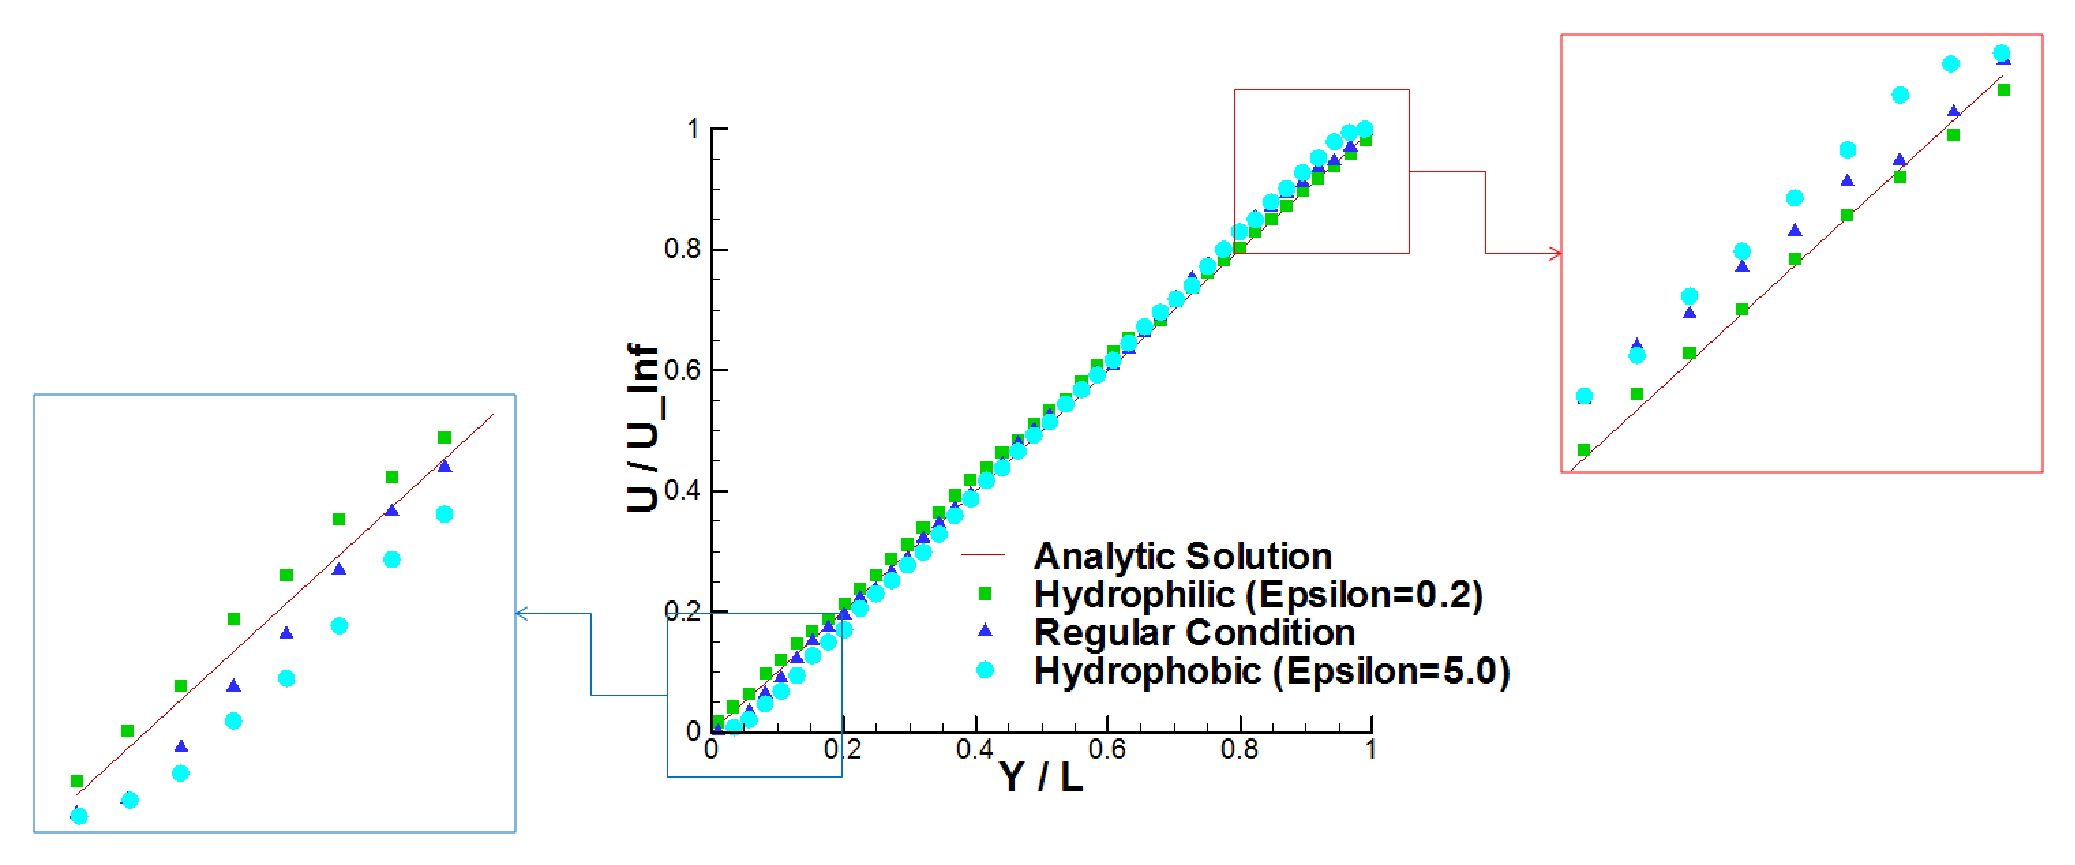
\includegraphics[width=0.9\linewidth]{MD_Solution.pdf}
\vskip-0.2cm
\caption{\small Steady Couette Flow Solution by Pure Molecular Dynamic Simulation; In normal condition (with the unique potential well depth between flow particle and surface material, denoted by $\epsilon$), the solution by MD is identical to the result of continuum approach. In hydrophobic case (smaller $\epsilon$) the fluid shows a slight slip on the wall, while the fluid particle strongly attempts to stick to the wall in hydrophilic case (bigger $\epsilon$).}
\label{MD_Solution}
\end{figure}


\skonote{Benefit over MD: efficient computational cost by CFD on global flow solution}

Context here...
\newline

\skonote{Raise unsolved issues and the necessity for parametric study in view of numerics}

Though the idea is novel and the approach is easy to follow, still a number of numerical issues are present on the implementation of hybrid CFD-MD simulation, especially for specifying coupling parameters. Layer size of data exchange zone with its position, sampling duration and the interval are major factors which affect the accuracy of coupled solution, and these conditions vary by the fluid and solid elements, flow condition and geometric characteristics. So far, there is no globally acceptable scheme for setting these coupling conditions. Thus, a number of experiments are required to empirically quantify (or mathematize) the coupling condition for specific problem.
\newline

\skonote{Issues of coupling on supercomputers: co-scheduling and load balancing. 2 paragraphs}

In addition to the physical and numerical interests of multi-physics coupled simulations, there also exist computational challenges of integrating multiple application domains into a single problem set. Considering very different computational kernels (one could be mesh-based, the other unstructured particle simulations) with very different computational time-scales, it is nearly impossible to incorporate distinct CFD and MD codes under the umbrella of a single tightly-coupled application (i.e., binding two application codes within a single MPI communicator). One possible alternative will be to implement coupling interface on individual code and control these logically separated codes as a virtually unified simulation package.
However, confined to parallel execution on conventional production system with batch queue, it cannot be guaranteed that two separate jobs will execute concurrently. Considering the computational characteristics of current application, where CFD and MD codes conduct frequent information exchange via their file interfaces, the first job to run will inevitably experience the idle waiting for its counterpart without the explicit support for co-scheduling. Another important challenge is the need for efficient load-balancing which takes into account the individual application's performance. Even if the two simulations could run concurrently, without explicit load-management/balancing support, there is likely to be inefficient utilization of compute resources due to load imbalance. As the performance of each simulation component changes with computing resource and problem size, re-adjustment of allocated resources to each task according to their performance is required during the simulation.
\newline

\skonote{Introducing what is a container job and what is its benefit: 1 paragraph}

Conceptually, the adoption of a Pilot-Job concept can be an answer to resolve above co-scheduling and load balancing issues of running a coupled multi-task simulation. The Pilot-Job is just a container task where a number of sub-tasks can run in a pre-defined schedule with the specified number of processors whether or not they are coupled. We basically devise this solution to overcome the concurrent scheduling requirement/constraints of coupled jobs; interestingly, the dynamic resource allocation capabilities of the Pilot-Job prove useful for the effective load-balancing of two independent but concurrently running codes. In contrast, if simulations were submitted as independent jobs, changing resource (CPU) allocation to address these changes is challenging -- as the change in resource assigned to one is correlated with a change in resource assigned to the other component.
\newline

\skonote{Tell the objectives of this research: Develop a Hybrid CFD/MD Simulation Framework including Domain Science Application Codes and Computational Framework. Mention that 'we basically used an in-house CFD code and famous LAMMPS MD package and modified both codes for coupled multi-physics simulation. We focus more on building an efficient coupled multi-task environment for hybrid CFD-MD simulation.' Also include the composition of chapters in the follow. 2 paragraphs}

Collectively, we are focusing on investigating numerical issues of applying the hybrid CFD-MD scheme to a nano-fluidic system, as well as designing and developing an efficient runtime framework for a coupled multi-component simulation. (What is our strength in physics?; We value our numerical experiments that this is the first trial to validate the hybrid CFD-MD approach in various system sizes and flow conditions. Also, our numerical simulation is the first trial to simulate innate unsteady flow using the current scheme.) In view of computational science, we believe our trial is the first documented utilization of Container-Job/Pilot-Job abstractions to perform coupled Multi-Physics simulations. We claim that there several distinct advantages that arise as a consequence of using Pilot-Jobs for Coupled Simulations: (i) obviates the need for a co-scheduler while preserving performance, (ii) enables dynamic resource allocation, which in turn is important for load-balancing across coupled simulations. %But given the lack of system or service-level support to address the challenges outlined above, there is a need to address the solution at the application level. This paper aims to provide novel solutions to the above problem using frameworks that are in user (application) space.

(Paper structure needs correction)
We begin the next section with an outline of the basic motivation and concept of coupled simulations. Numerical details of individual code and implementation of hybrid scheme are presented in the next Section. Validation of coupled simulation package and its application to other problems follow in Section 4. Couette flow simulation and Stokes boundary layer problems are conducted on two different system scales. Hybrid layer size and sampling duration along with sampling interval, are discussed. The summary of our work and the future plan are expressed in Section 5.
\newline



% -------------------------------------------------------------------------
\section{A Hybrid CFD-MD Approach - Numerical Technique for Multi-scale Flow Simulation}


\skonote{About previous works: 2 paragraphs (More$^5$ details!)}

The study of microfluidic mechanism including from nanoscale fluidic system to continuum one has been recently developed using hybrid CFD-MD method. The hybrid method is taking the advantage of each atomistic and continuum descriptions adopting information exchange based on constrained equation of motion over the overlap region~\cite{Thompson},\cite{Nie},\cite{Yen},\cite{Steijl}. Modification for mutual flux exchange across the domain boundary has been proposed~\cite{Flekkoy},\cite{Wagner} and more studies about the flux exchange scheme~\cite{Hadjicon1},\cite{Hadjicon2}, coupling parameters~\cite{Wang} have been accomplished. However, more challenging point of view are still remaining such as extreme physical domain condition, explicit time duration of passing information, the region for taking the statistics of atomistic averaging and others.
\newline

\skonote{Their limitations: 1 paragraph. For example, lack of application problems, unclear setup of coupling conditions, etc.}

Context here...
\newline

\skonote{How to Couple: Schematic of CFD and MD zones. 1 paragraph.}
% The hybrid CFD/MD approach is a simulation method which adopts the continuum hypothesis in capturing macroscopic features of a flow-field and details atomistic intermolecular interactions on interfaces of different materials by using the MD approach. CFD can accurately predict flow properties on conventional moderate/large size fluid domains, but is intrinsically impossible to reflect characteristics of surrounding solid materials within a interfacial region. While standard classical MD can provide atomistic level resolution of interactions between particles, it becomes computationally demanding as the size of simulated system grows. So, neither method is suitable for solving a mesh-scale fluid system where the viscous effect dominates the flow characteristics but macroscopic features are also worth capturing efficiently. The best solution would be, as can be seen in Fig.~\ref{Fig:Couette}, to carry out the hybrid CFD/MD approach with which atomistic interactions between solid elements and fluid particles near the wall is simulated by MD and the macroscopic flow field is calculated by CFD.

(More details)
The hybrid CFD-MD approach basically starts from the concept that the inertial force from macroscopic flow domain dominates the system while intermolecular effect cannot be negligible in the low-speed flow region. As given in Fig.~\ref{Fig:Couette}, CFD approach analyzes the macroscopic flow characteristics with the moderate flow velocity, while MD independently solves low-speed flow region. These two domains overlap in the middle, where CFD and MD exchange their solutions.
\newline

\skonote{Meaning of each layer within overlap region. 1 paragraph.}

(Mention the meaning of the buffer and decision of their sizes as well: at least it should be longer than Van der Waals cutoff length. Don't mention 'Van der Waals' here! Change the expression like, 'information from CFD and MD should not conflict each other at the same time')
In the CFD-MD hybrid overlap region, computational domain can be decomposed into three interesting regions. Applying external force region where located uppermost boundary of overlap region and in order to the momentum continuity between two approaches. The hybrid schemes have to exchange their information at the overlap region between the different approaches. The way passing information from MD to CFD is more clear since the averaging of particle information applies to a macroscopic state of CFD. While passing information from macroscopic CFD to MD has difficulty and it demands a constrained particle dynamics to achieve consistence between two different multi-scale approaches.
\newline

\skonote{Nayong: Can you change the 'Stationary lowermost wall' to 'creeping flow or stationary wall'?}


%%%%% FIGURE %%%%%
\begin{figure}
\centering
%\vspace{-1em}
%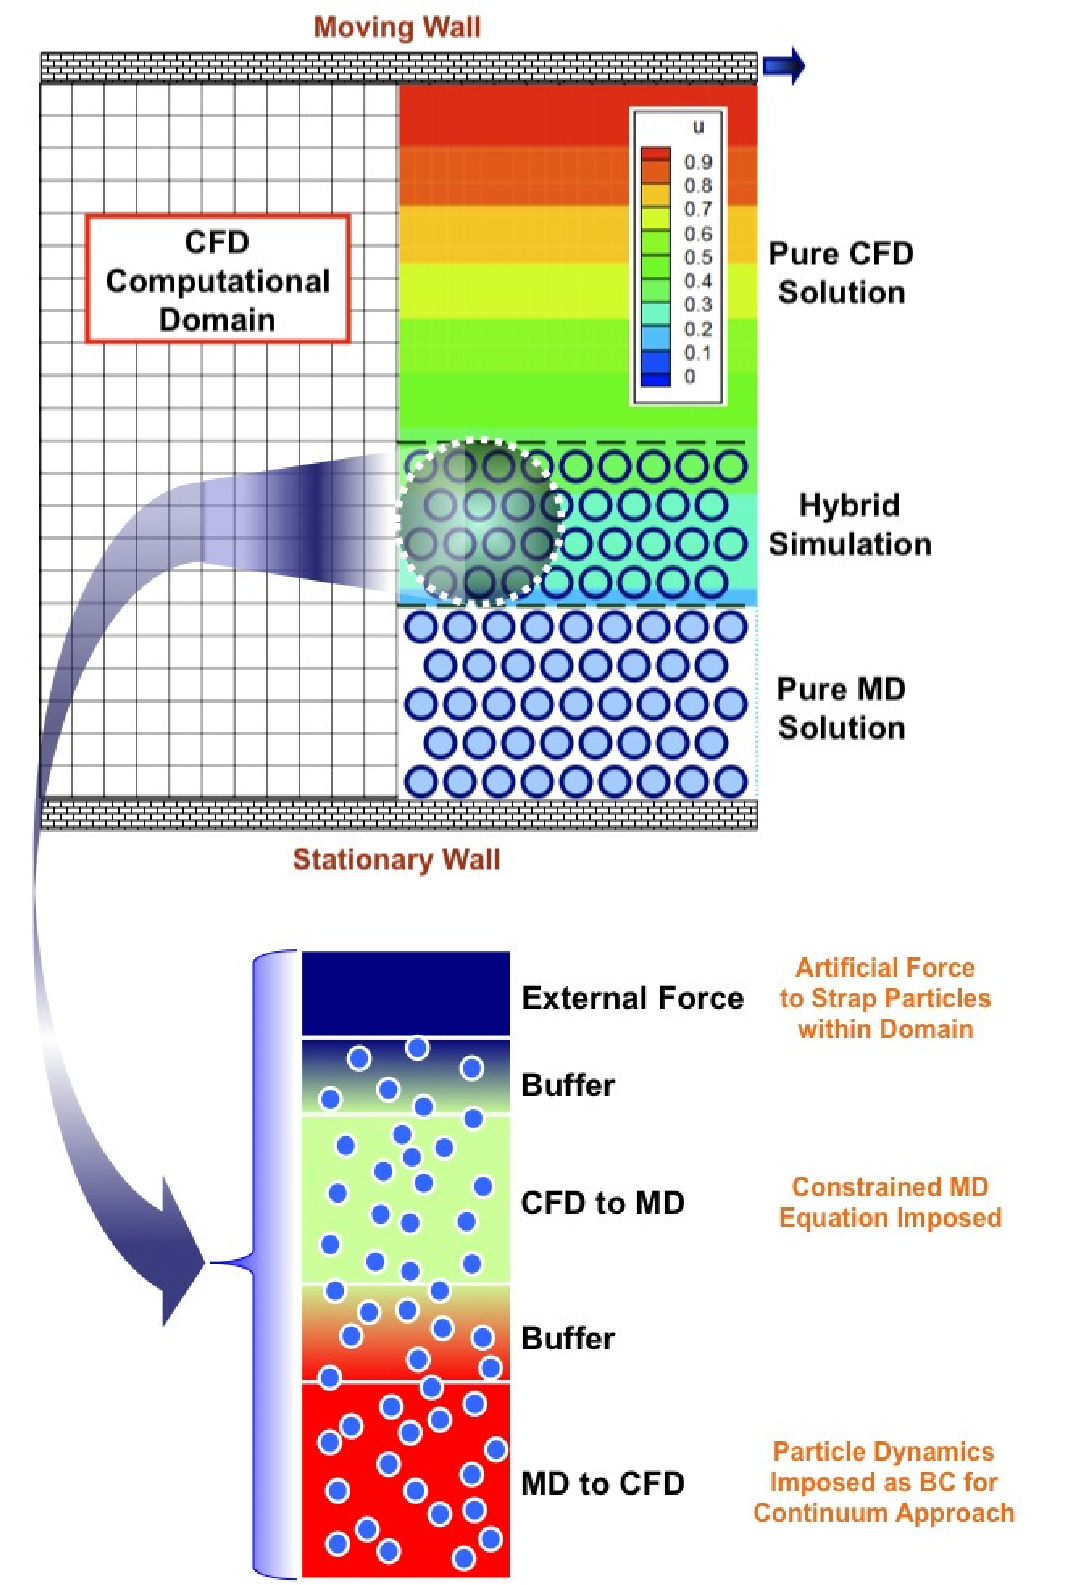
\includegraphics[scale=0.5]{fig1.pdf}
%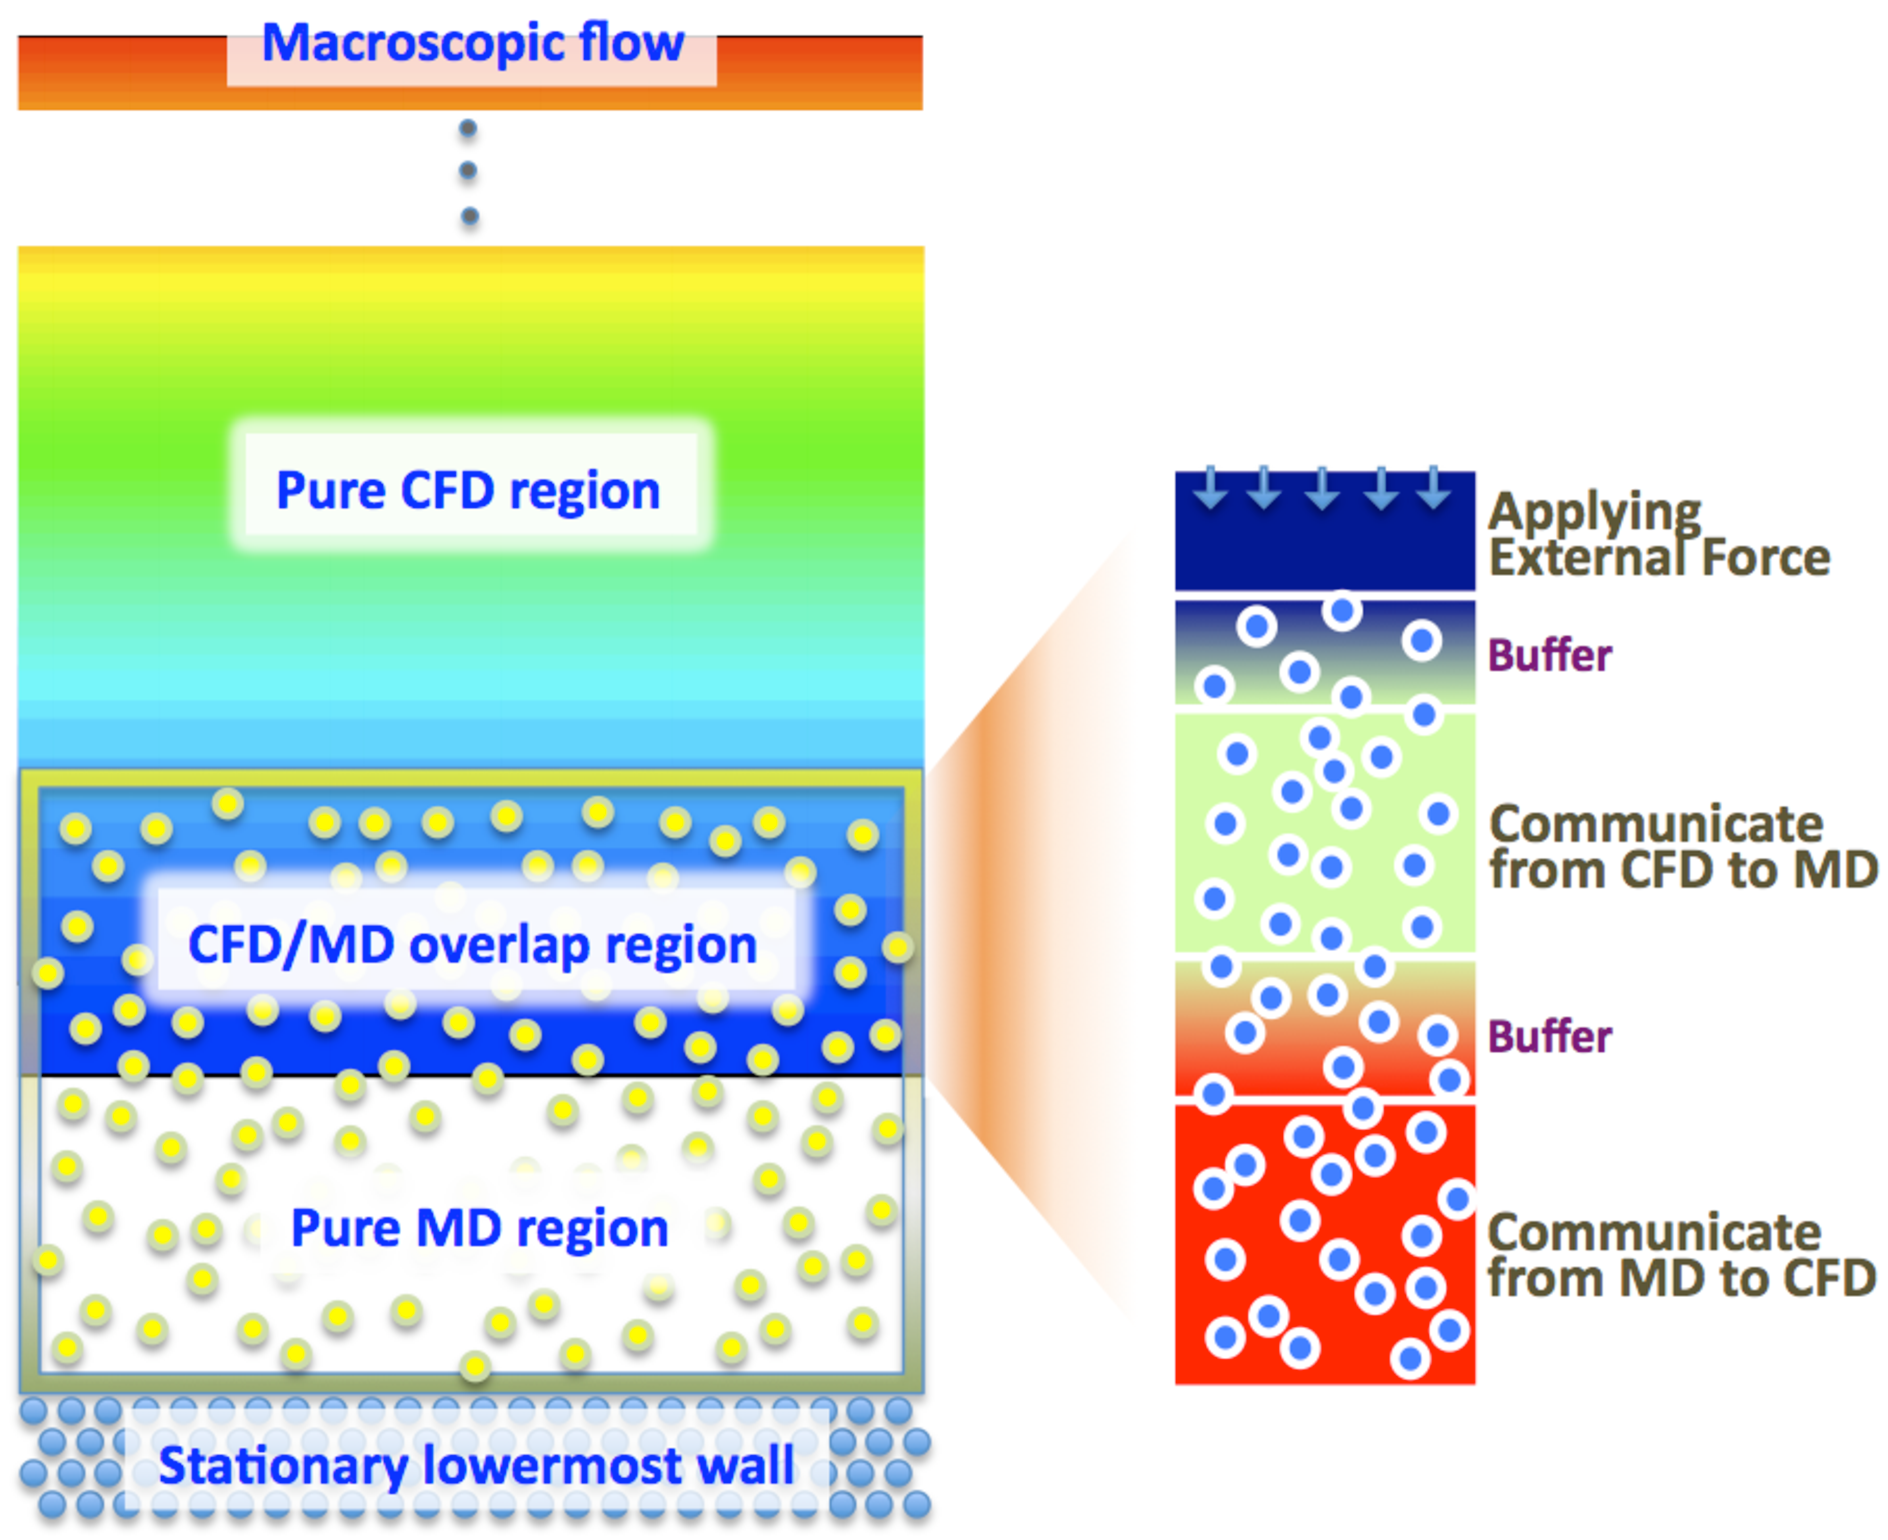
\includegraphics[scale=0.3]{Couette7.pdf}
%\linebreak
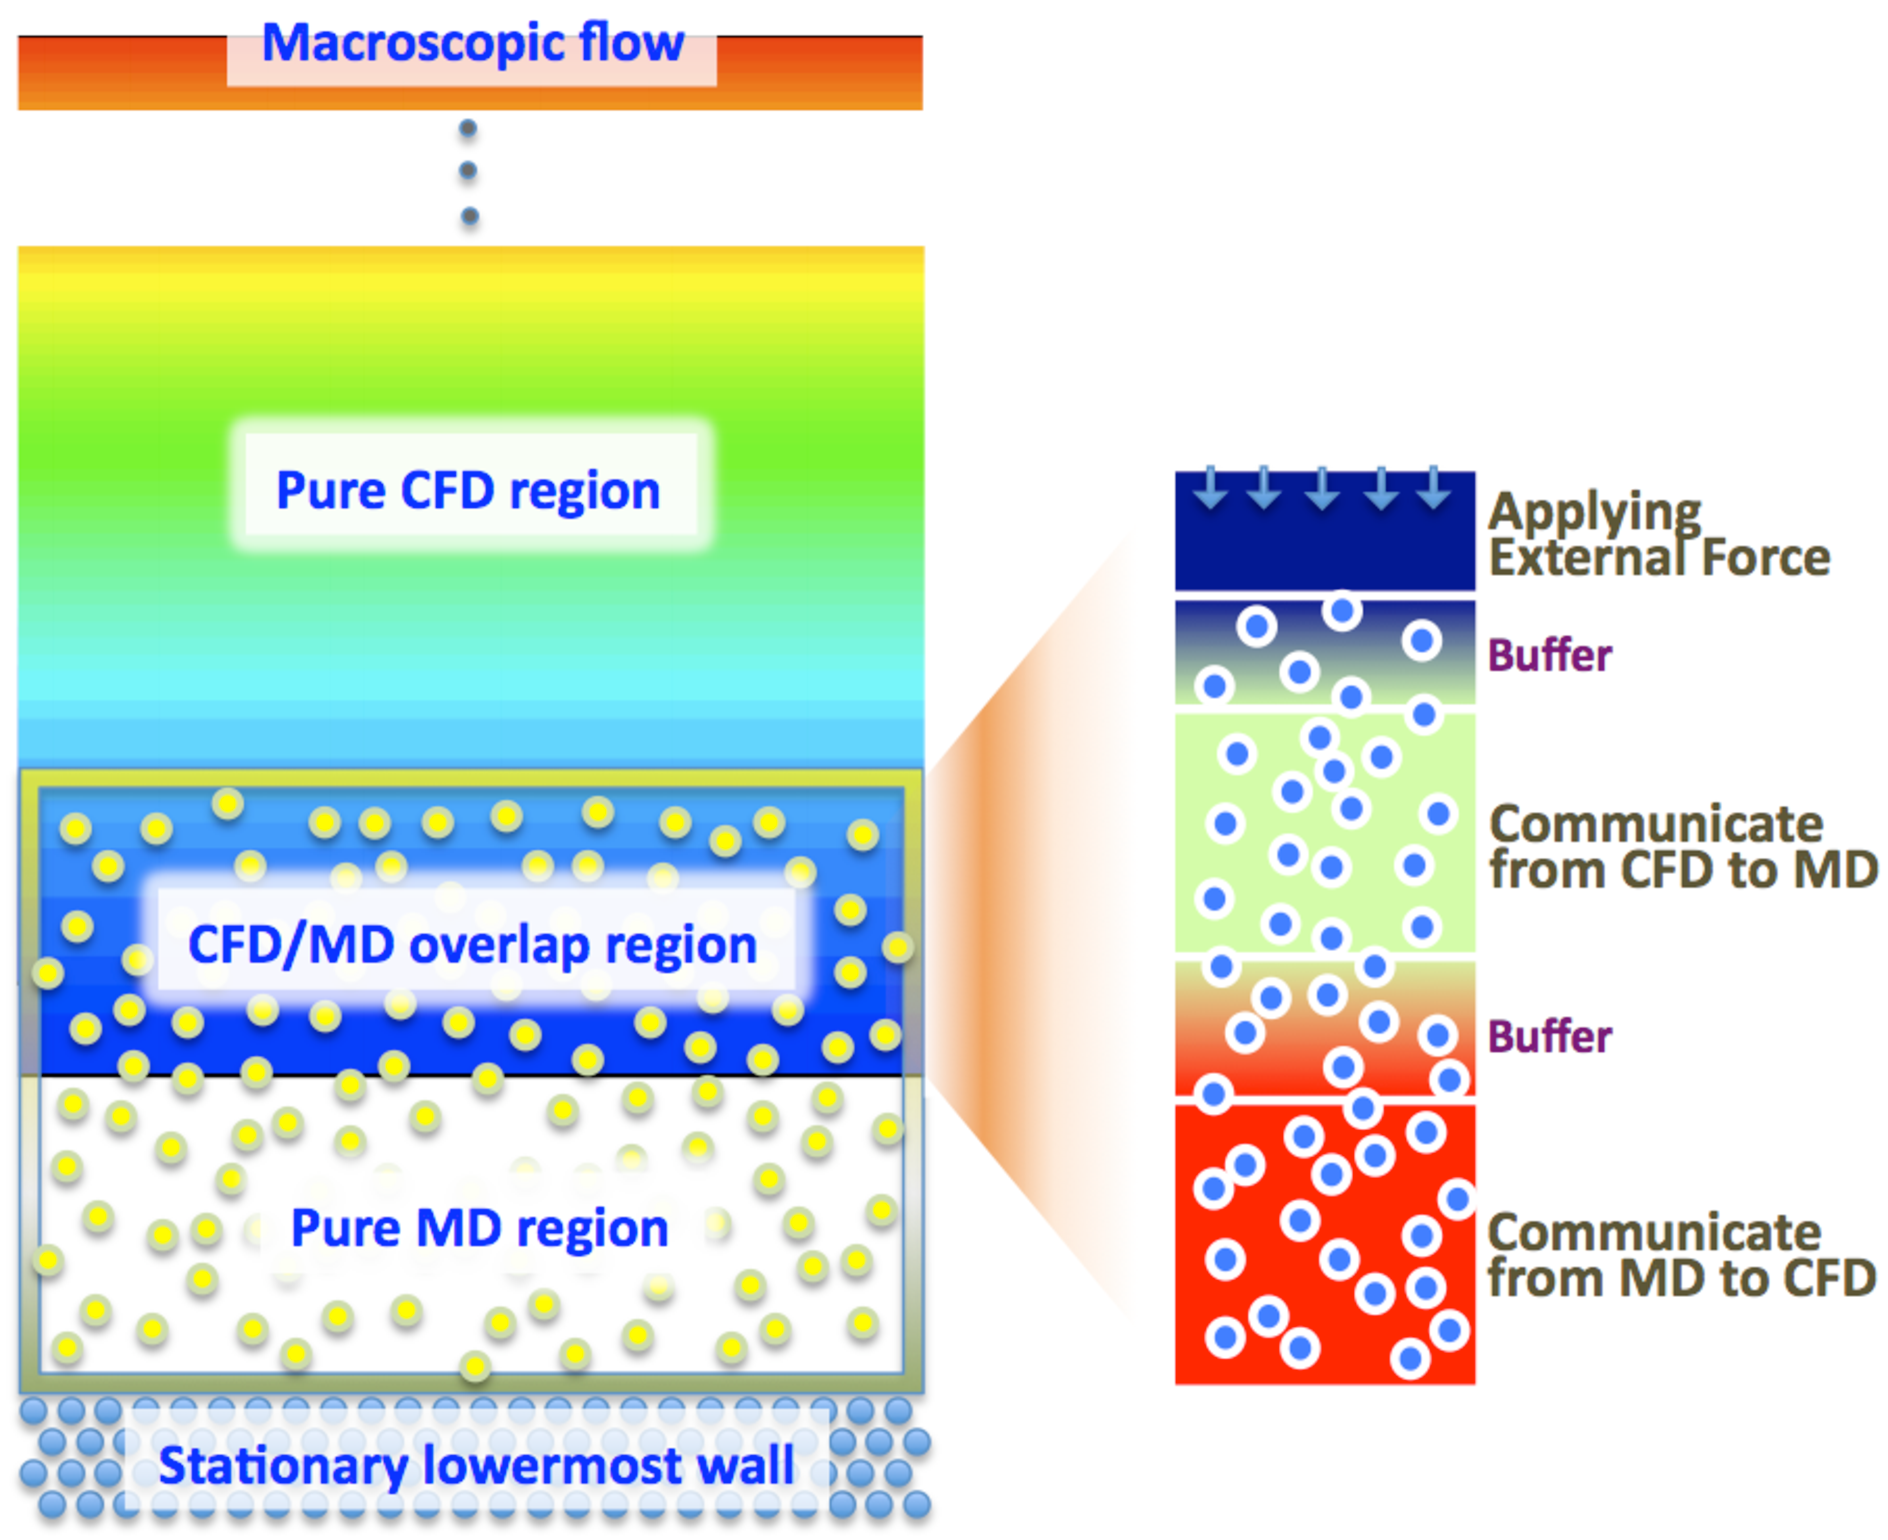
\includegraphics[width=0.8\linewidth]{Couette7.pdf}
\vskip-0.2cm
\caption{\small Schematic Diagram of the Hybrid Domain with Detailed View of Overlapping Zone; Overall continuum/atomistic computational domain including overlap region is shown on left figure. Detailed layer by layer explanation of overlapping region is indicated by right figure.}
\label{Fig:Couette}
%\vspace{-1em}
\end{figure}
%%%%% FIGURE %%%%%



\section{SAGA and SAGA-based Frameworks - An Efficient Runtime Environment for Coupled Multi-component Computations}

\skonote{Introduction to SAGA: *** paragraphs as you like :)}

The Simple API for Grid Applications (SAGA) is an API standardization effort within the Open Grid Forum (OGF)~\cite{ogf_web}, an international standards development body concerned primarily with standards for distributed computing. SAGA provides a simple, POSIX-style API to the most common Grid functions at a sufficiently high-level of abstraction so as to be independent of the diverse and dynamic Grid environments. The SAGA specification defines interfaces for the most common Grid-programming functions grouped as a set of functional packages (Fig.~\ref{Fig:SAGA1}). Some key packages are:

\begin{figure}
 \begin{center}
     \includegraphics[width=0.40\textwidth]{stci_saga_figures-1.eps}
 \end{center}
\caption{\small Layered schematic of the different components of the SAGA landscape. At the topmost level is the simple integrated API which provides the basic functionality for distributed computing. Our BigJob abstraction is built upon this SAGA layer using Python API wrapper}
 \label{Fig:SAGA1}
 \vspace{-1em}
\end{figure}

\begin{itemize}
\item File package - provides methods for accessing local and remote filesystems, browsing directories, moving, copying, and deleting files, setting access permissions, as well as zero-copy reading and writing
\item Job package - provides methods for describing, submitting, monitoring, and controlling local and remote jobs. Many parts of this package were derived from the largely adopted DRMAA %~\cite{drmaa_url} specification.
\item Stream package - provides methods for authenticated local and remote socket connections with hooks to support authorization and encryption schemes.
\item Other Packages, such as the RPC (remote procedure call) and Replica package
\end{itemize}


\skonote{Introduction to BigJob and related researches from other researchers: show their limitation as well - i.e., LB issue, etc.. Include REMD, co-scheduling of multiple tasks via SGE in Ranger. 2 paragraphs. I'd like to include "SAGA enables creation of higher levels of abstraction, such as a container-job or a Pilot-Job (which, as we will discuss, is referred to as the BigJob~\cite{saga_royalsoc}). The SAGA-based Pilot-Job is infrastructure neutral, unlike {\it all} other Pilot-Jobs."}

\skonote{Exclude the mention about the multiple BigJobs. Also, focus on explaining BigJob's advert service module in detail, including referring to Andre's paper}

Fig.~\ref{Fig:BigJob_Structure} shows the structure of BigJob and its operation flow. When a BigJob is submitted to the remote resource, the application manager monitors the status of this pilot-job through the advert service. When resources are allocated to the BigJob, the application manager allots the obtained resources to its sub-jobs and a coupled simulation starts under the control of a multi-physics agent in the remote resource. Advert service keeps on getting the status of a pilot-job from the queuing system and the status of sub-jobs from multi-physics agent and also delivers this information to the application manager by a push-pull mechanism. The application manager watches the status of sub-jobs and decides the next event when the coupled simulation is finished. When one default BigJob is launched, sub-jobs keeps running until final solution is achieved and the manager quits the Pilot-Job at that time. In case multiple BigJobs are submitted for the same simulation or if a load balancing function is included, sub-jobs experience several restarts from their checkpointing data, reflecting changed processor allocation to each application. In the former case, resource allocation to each sub-job follows a pre-defined map according to the number of BigJobs allotted to the simulation; in the latter case, resource allocation to each sub-job becomes dynamic according to its performance, as discussed in the next section.


%%%%% FIGURE %%%%%
\begin{figure}
\centering
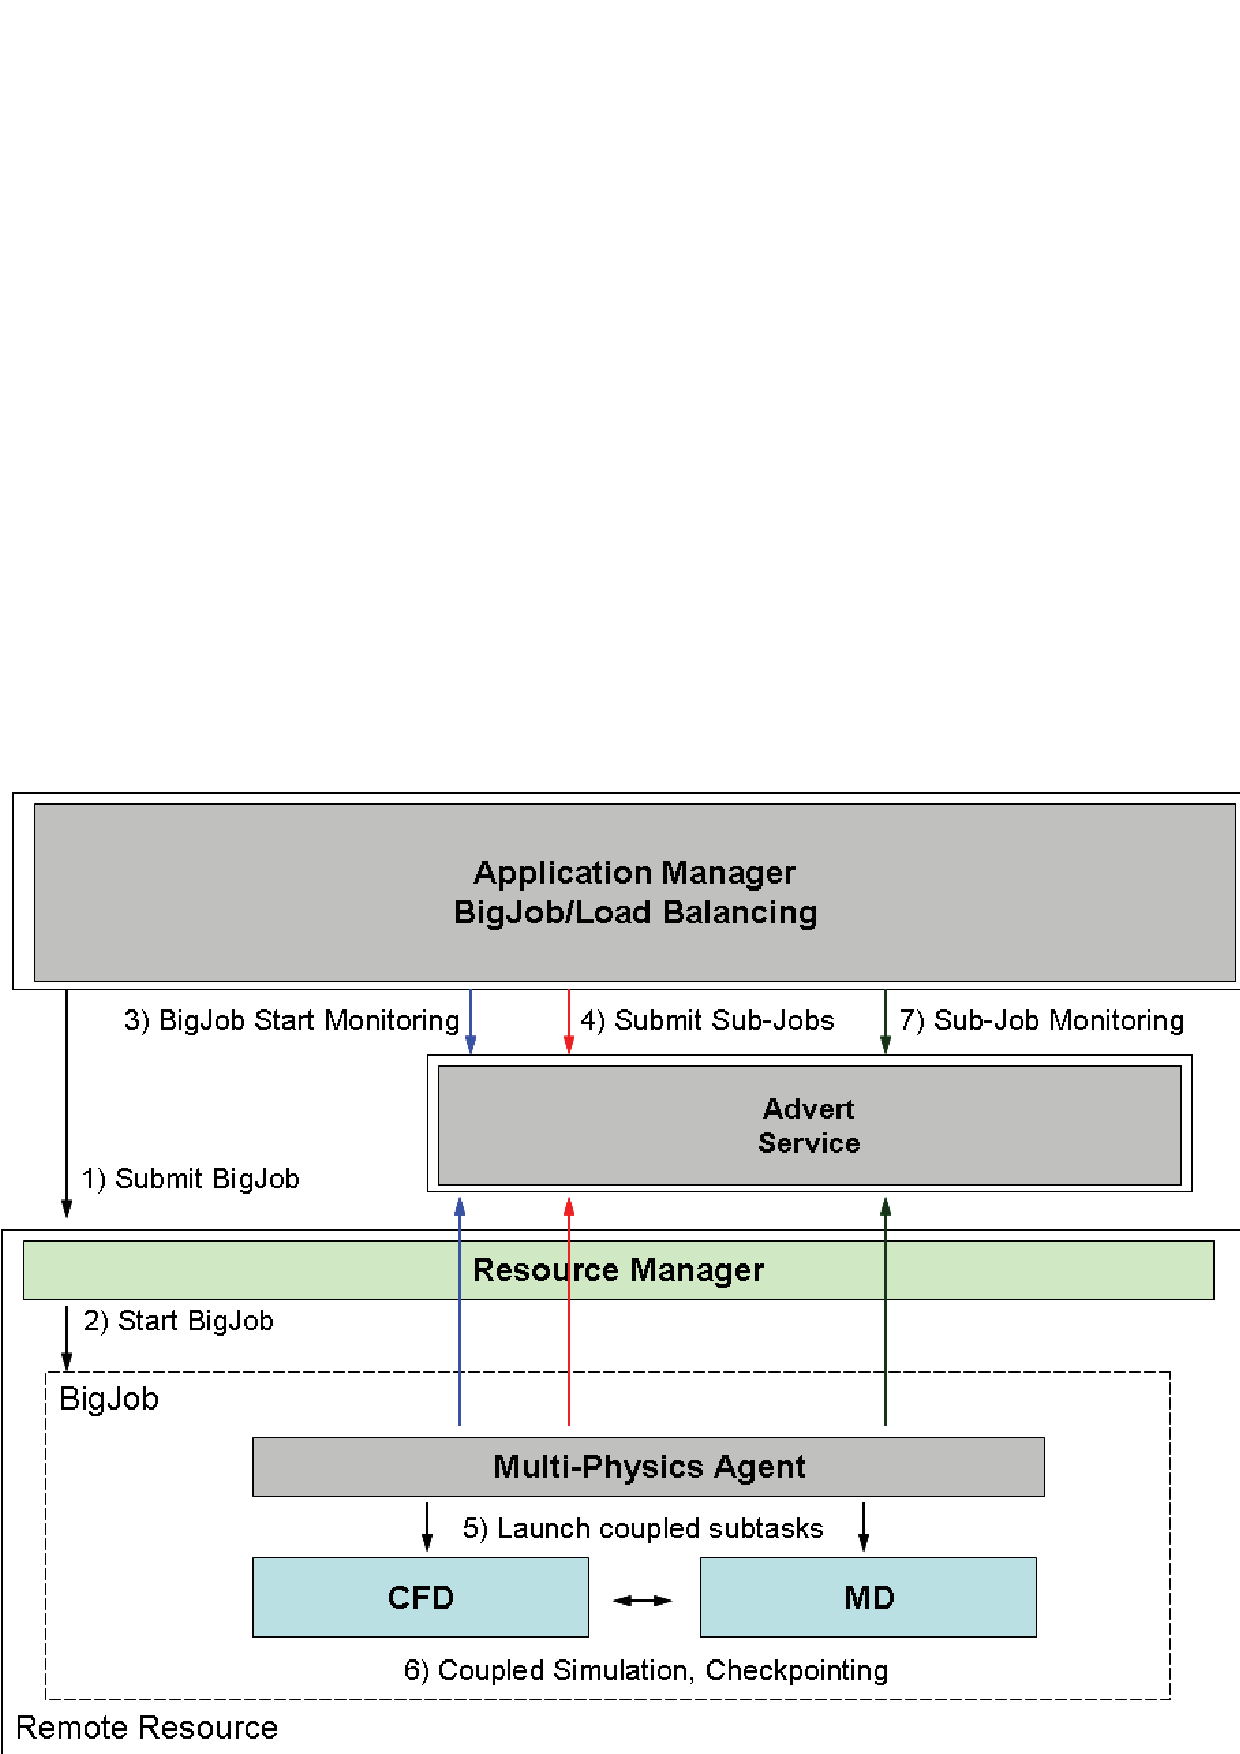
\includegraphics[scale=0.38]{Structure_of_BigJob}
\caption{\small Architecture of the Controller/Manager and Control Flow: Application manager is responsible for job management including BigJob and sub-job submission, their status monitoring functions. We implement a load balancing module, and migration service based on job information. Application agent system resides on each HPC resource and conducts job information gathering and also communicates with the application manager via the advert service}
\label{Fig:BigJob_Structure}
\vspace{-1em}
\end{figure}
%%%%% FIGURE %%%%%



\section{Development of A Hybrid CFD-MD Simulation Toolkit}

\subsection{Features of Baseline CFD and MD Codes}

\skonote{I'll also include 'What is continuum hypothesis and how small is the acceptable range.'}

Two-dimensional unsteady incompressible Navier-Stokes equations are chosen for governing equations to solve the nano-scale flow:

\vskip-.6cm
\begin{eqnarray}
\frac{\partial {u}_{i}}{\partial {x}_{i}} = 0
\end{eqnarray}
\vskip-.6cm
\begin{eqnarray}
\frac{\partial {u}_{i}}{\partial t} + \frac {\partial} {\partial {x}_{j}} ({u}_{i}{u}_{j}) = -\frac {\partial p} {\partial {x}_{j}} + \nu \frac {{\partial} {u}_{i}} {\partial {x}_{j} \partial {x}_{j}} \nonumber
\end{eqnarray}
where $\nu$ is the kinematic viscosity.

%The primary difficulty in solving the incompressible Navier-Stokes equations in primitive variables stems from the lack of a time derivative in the continuity equation. There is no straightforward way to iteratively march these equations in time and ensure a divergence-free velocity field.
%In this work, we adopted the pseudo-compressibility method$^{\cite{PseudoCompressibility}}$ to form a hyperbolic system of equations which can be marched in pseudo-time to a steady-state solution. The method can also be extended to solve time-dependent problems by using sub-iterations in pseudo-time at each physical time step. A time derivative of pressure is added to the continuity equation resulting in

In this work, we adopted the pseudo-compressibility method~\cite{PseudoCompressibility} to form a hyperbolic system of equations which can be marched in pseudo-time. A time derivative of pressure is added to the continuity equation resulting in

\vskip-.6cm
\begin{eqnarray}
\frac{\partial (p/\rho)}{\partial \tau} = - \beta \frac{\partial {u}_{i}}{\partial {x}_{i}}
\end{eqnarray}
where $\beta$ denotes a pseudo-compressibility parameter, currently set up as 2.5.

For time-accurate unsteady simulation, dual time stepping method is adopted and it is combined with the LU-SGS (Lower-Upper Symmetric Gauss-Seidel) scheme~\cite{LU-SGS} for the implicit time integration. The inviscid fluxes are upwind-differenced using Osher's flux-difference splitting scheme~\cite{Osher}. For higher-order spatial accuracy, the MUSCL (Monotone Upstream-centered Schemes for Conservation Laws)~\cite{MUSCL} approach is used on inviscid flux calculation. Viscous fluxes are calculated using the conventional second-order central differencing.

Molecular dynamics (MD) computer simulation technique is a specified computer simulation method for molecular systems, including microscopic details of a system and macroscopic statistical properties, which are the properties of the atoms, the interactions between particles, molecular characteristics, structure of molecules, transport phenomena etc.~\cite{Allen},\cite{Haile},\cite{Rapaport} In molecular dynamics, an initial velocity is assigned to each atom, and Newton's laws are employed at the atomic level to propagate the system's motion through time evolution:

\vspace{-.2em}
%\footnotesize
\begin{equation}
F_{i} = m_{i}a_{i}
\label{eq:Newton}
\end{equation}
\normalsize
here each atom $\it i $ in a system constituted by N atoms, mi is the mass of i$^{th}$ atom, ai is the acceleration and denote by $\it {d^2r_{i}} / {dt^2}$, and $\it F_{i}$ is the force on i$^{th}$ atom, due to the atomic interaction which is calculated based on the potential energy between individual particles.
The simplest choice for the potential energy $\it U(r)$  can be written as the sum of pairwise interactions of particles:

\vspace{-.2em}
%\footnotesize
\begin{equation}
U(r_{1}, ...  ,r_{N}) =  \displaystyle\sum_{i} \displaystyle\sum_{j>i}  u(|r_{i} - r_{j}|)
\label{eq:PEnergy}
\end{equation}
\normalsize
where $\it i$ and $\it j$ particles are located at $r_{i}$ and $r_{j}$, and only $\it j>i$ cases have been considering for each particles pair once.
The most commonly used two-body interaction model is the Lennard-Jones (12-6) potential is applied to calculate pairwise interaction and is define as:

\vspace{-.2em}
%\footnotesize
\begin{equation}
 u(|r_{i} - r_{j}|) = 4\epsilon_{ij}[(\frac{\sigma_{ij}}{r_{ij}})^{12}-(\frac{\sigma_{ij}}{r_{ij}})^{6}]
 \label{eq:LJ12}
\end{equation}
\normalsize
where $\epsilon_{ij}$ and $\sigma_{ij}$ denote the pairwise potential well depth and the atom size parameter respectively, and $\it r_{ij}$ is the distance between the particle $\it i$ and $\it j$.
The term $\it 1/r_{ij}^{12}$ dominating at short range distance repulsive behavior based on the Pauli principle to avoid overlapping the electronic clouds when particles are  brought very close to each other. The term $\it 1/r_{ij}^6$ dominates at long range attractive forces by van der Waals dispersion forces.

The time integration algorithm is required to integrate the equation of motion of the interacting particles and computing molecular trajectories, one of most common velocity Verlet algorithm is employed to compute the simulation.
In this work,  the MD simulations were performed by using the modified version of Large Atomic Molecular Massively Parallel Simulator(LAMMPS). It is the classical molecular dynamics open software written in C++ and developed by Sandia National Labs.~\cite{LAMMPS}


\subsection{Implementation of Hybrid Schemes}

\skonote{Numerical modeling and implementation on each solver. 3 paragraphs. Start with external force layer: specify the equation, mention that 'this artificial force modeling is implemented on MD package, to trap escaping particles within the computational domain'. Next paragraph about CFDtoMD: Discuss the meaning of constrained MD equation and specify how the code is changed, mention that 'this constrained MD equation specifies that particles in this layer eventually follow the averaged flow speed from the continuum approach.' Last paragraph about MDtoCFD: express that the average of particle velocity in this layer is applied to CFD's boundary condition, changing the CFD code. Nayong: Can you state that 'external force is numerical treatment, while CFDtoMD is physical term to follow the averaged velocity from macroscopic profile'?}

CFD-MD hybrid method has numerical strategy for file-based information exchange between continuum description for macroscopic scale and discrete particle description for microscopic scale. For this information exchange, both codes have the file interface, where each writes the velocity profile of overlapping region, waits for its counterpart's velocity data and receive the data as a boundary condition in the overlap region.
\newline

\skonote{a little more detail: clearly specify and refer to zonal distribution in Fig.~\ref{Fig:Couette}}

Additional change made on CFD code is the implementation of overlapping scheme, in the same way as Chimera overset mesh~\cite{Chimera}. That is, pure MD region is declared as holes and MD boundary layers are treated as fringe cells. Averaged particle velocity over time interval at MDtoCFD region (see Fig.~\ref{Fig:Couette}) from molecular dynamics domain is stated as fringe boundary condition to the CFD code.

On the other hands, MD code experiences a lot of change to implement hybrid scheme. First, the external force should be imposed to prevent leaving particles from the control domain and the force is applied its perpendicular relative position of uppermost MD layer, as was seen in Fig.~\ref{Fig:Couette}.

\vspace{-.2em}
%\footnotesize
\begin{equation}
 F_{ext, i} = -p_{a}\sigma\frac{y_{i}-Y_{n-1}}{1-(y_{i}-Y_{n-1})/(Y_{n}-Y_{n-1})}
 \label{eq:Con_vel}
\end{equation}
\normalsize
where $\it p_{a}$ denote the average pressure in the MD region, $\it Y_{n}-Y_{n-1}$ is the thickness of the uppermost layer which is applied the force and $\it F_{ext}$ is the external force acting on $\it i_{th}$ particle located on position $\it y_{i}$.

Communicate MD information to CFD can be achieved uncomplicated since the coarse grained microscopic information in time is imposed to macroscopic resolution of the continuum domain. The reverse procedure, to implement  CFD to MD communication, is more difficult and requires artificial intervention to maintain mass and momentum conservation. The average velocities of particles in $\it J_{th}$ cell is equal to the velocity $\it u_{J}$ in continuum cell.

\vspace{-.2em}
%\footnotesize
\begin{equation}
 u_{J}(t) = \frac{1}{N_{J}} \displaystyle\sum_{i} v_{i}
 \label{eq:Con_vel}
\end{equation}
\normalsize
where $\it v_{i}$ is velocity of  $\it i_{th}$ particle and $\it N_{J}$ is the number of particles in the cell.   With taking Lagrangian derivative  of eq.~\ref{eq:Con_vel},

\vspace{-.2em}
%\footnotesize
\begin{equation}
 \frac{Du_{J}(t)}{Dt} =  \displaystyle\sum_{i} \frac{\ddot{x_{i}}}{N_{J}}
 \label{eq:Lagrangian}
\end{equation}
\normalsize
The Classical MD equation of motion can be generalized to obtain constraint by adopting the fluctuation in acceleration of each particles, $\zeta_{i}$

\vspace{-.2em}
%\footnotesize
\begin{equation}
 \frac{F_{i}}{m_{i}} = \ddot{x_{i}}(t)  =   \frac{Du_{J}(t)}{Dt} + \zeta_{i} = \frac{\displaystyle\sum_{i}F_{i}(t)} {\displaystyle\sum_{i}m_{i}} +   \zeta_{i}
 \label{eq:Con2}
\end{equation}
\normalsize
where $\it F_{i}$ is the force on $\it i_{th}$ particle based on the interactions between particles,  $\it m_{i}$ is mass of each atom and  eq.~\ref{eq:Con2} satisfies,
\vspace{-.2em}
%\footnotesize
\begin{equation}
\displaystyle\sum_{i}\zeta_{i}m_{i} = 0
 \label{eq:Con2}
\end{equation}
\normalsize
The constrained particle dynamics with conventional equation of motion can be written as:

\vspace{-.2em}
%\footnotesize
\begin{equation}
 \ddot{x_{i}}(t) = \frac{F_{i}}{m_{i}} -  \frac{\displaystyle\sum_{i}F_{i}(t)} {\displaystyle\sum_{i}m_{i}} - \frac{1}{\Delta t_{MD}} \{  \frac{\displaystyle\sum_{i}m_{i}\dot{x_{i}}} {\displaystyle\sum_{i}m_{i}} - u_{J}(t + \Delta t_{MD})\}
 \label{eq:Con3}
\end{equation}
\normalsize
The continuum velocity and the mean microscopic velocity from MD over control domain provide the synchronization of the mass and momentum consistent via eq.~\ref{eq:Con3}.



Figure~\ref{Hybrid_Timescale} shows the schematic view of synchronization mechanism between CFD and MD domains. When both solvers approach the data exchange point (denoted by $t-{\Delta}t$), they exchange the information in the overlapping region and advance to the next exchange point ($t$). In the data exchange point, CFD sends the velocity profile at that instance. On the other hand, MD sends averaged velocity over a finite time duration ($S_{MD}{\times}{\Delta}t$). In MD simulation, spatially averaged velocity at an instance contains very high noise, thus it is inevitable to average particles' velocities over time. Data exchange interval (${\Delta}t$) is set sufficiently large compared to the averaging duration.

This mechanism gives us a better parallel efficiency compared to conventional sequential coupling mechanisms where one domain advances to the next exchange point and leads its counterpart to approach this point.~\cite{Time_Mechanism} As they send and receive their flow data at the same point, both codes can independently advance to the next time level without a large computing cost on waiting. So, parallel performance can ideally reach the single code running only if an appropriate load balancing between two domains can be applied. However, we should agree that this approach inherently includes the time lagging in CFD-MD boundary zone, because averaged molecular dynamic velocity over backward time scale is represented as the solution at that instance.
% Additionally, in any algorithm, codes experience the time lagging due to the impose of explicit BC in the hybrid domain.

\begin{figure}[ht]
\centering
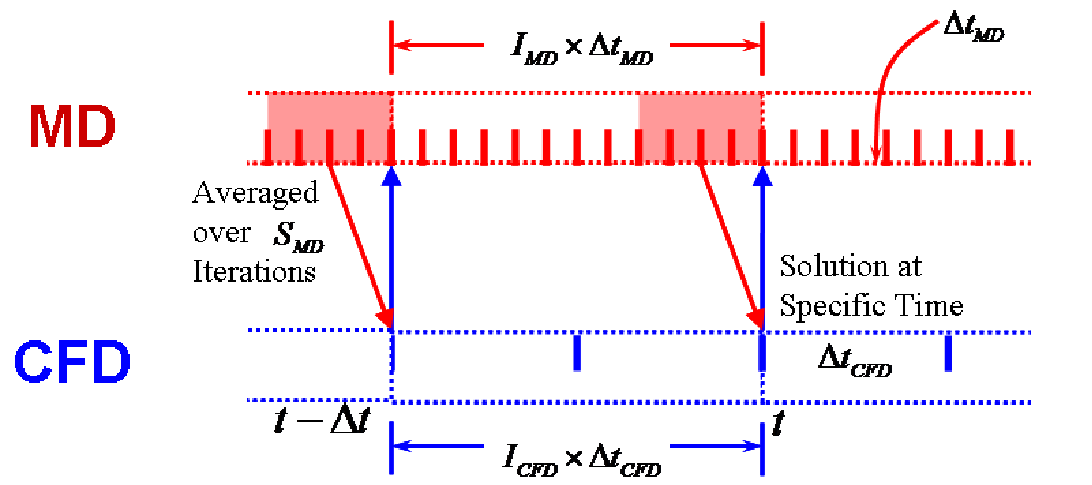
\includegraphics[width=0.7\linewidth]{Hybrid_Flowchart_1.pdf}
\vskip-0.2cm
\caption{\small Time Evolution Mechanism of Application Codes; CFD and MD codes are scheduled to conduct data exchange in the overlapping region at every $\Delta{t}$ time. CFD and MD solvers do sub-iterations until approaching the next data exchange point, by $I_{CFD}$ and $I_{MD}$. CFD solution at $t-\Delta{t}$ is directly applied as the boundary condition for MD simulation from $t-\Delta{t}$ to $t$, while averaged molecular dynamic velocity on $S_{MD}\times\Delta{t_{MD}}$ durations are imposed as CFD boundary conditions at this time instance.}
\label{Hybrid_Timescale}
\end{figure}



% Figure~\ref{Hybrid_Flowchart} denotes overall flowchart of CFD and MD solvers. Until they reach the file exchange point, both codes independently run their solution procudure. At the data exchange point, both codes first send the data and wait for receiving.

%
%\begin{figure}[ht]
%\centering
%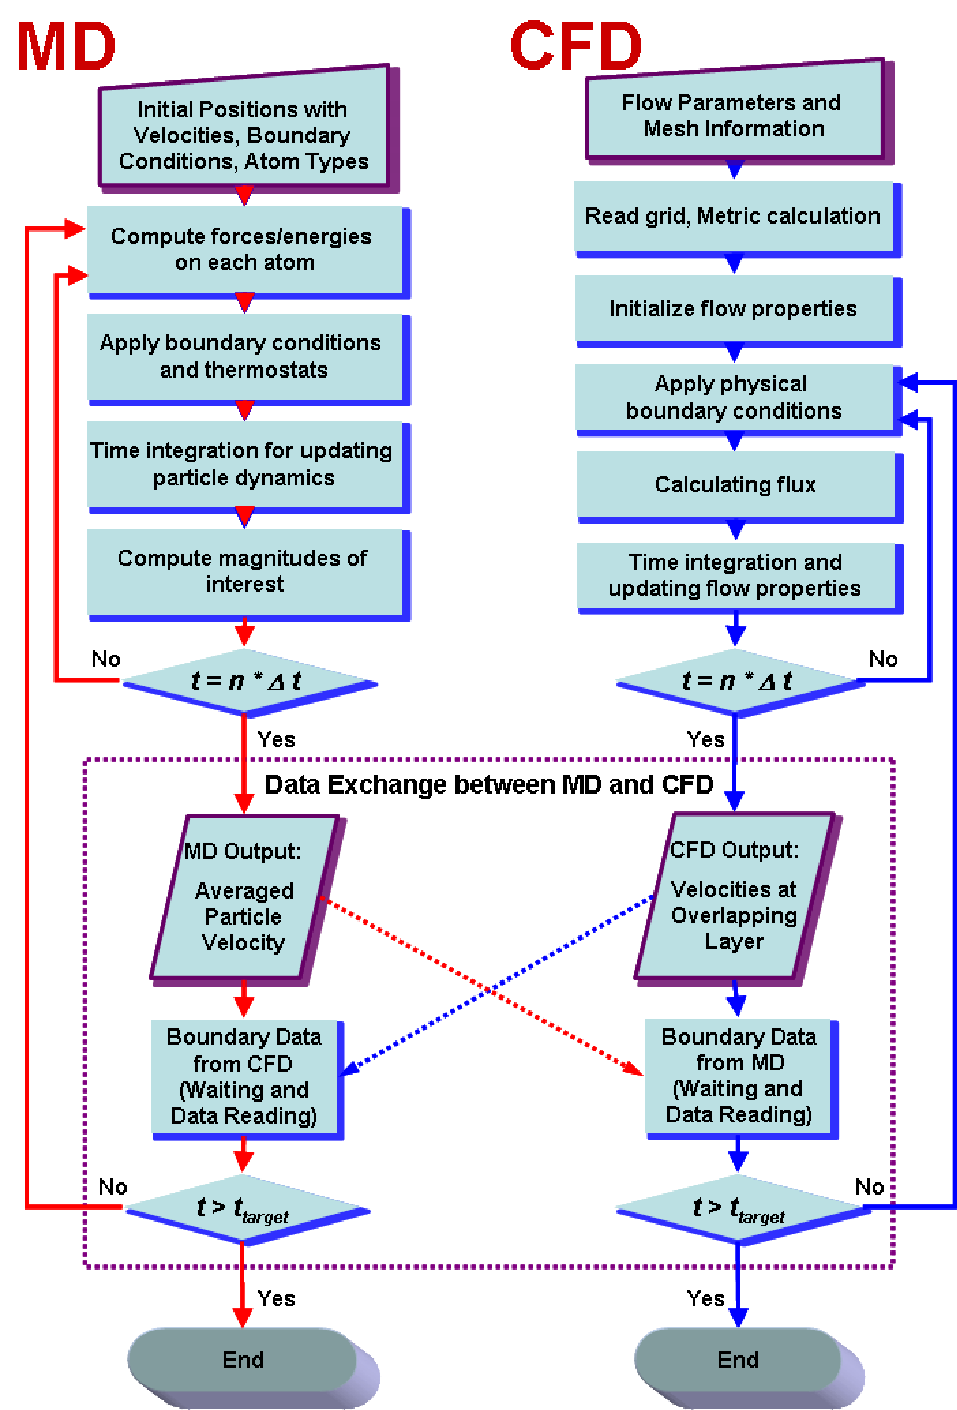
\includegraphics[width=0.6\linewidth]{Hybrid_Flowchart_2.pdf}
%\vskip-0.2cm
%\caption{Flowchart of Coupled Codes; CFD and MD codes have the identical flowchart except the information exchange between two codes and the additional consideration of a hybrid boundary condition. On every data exchange period, both codes first write their flow properties in the hybrid region and wait for the datafile from their counterpart. As they exchange their flow data at the same time level, they can concurrently advance to the next time level without a large computing cost on waiting for data exchange.}
%\label{Hybrid_Flowchart}
%\end{figure}



\section{Construction of a Coupled Multi-physics Simulation Framework}

\subsection{Load Balancing for Coupled Multi-Physics Simulation}

The flexibility to re-distribute resources (processors) to the individual task does not imply efficient utilization. This is the responsibility of a load-balancer (LB). We will discuss the implementation and algorithm of this LB~\cite{Ko}; it is important to mention that the LB functions in the context of the SAGA-BigJob framework.
Each application's load is determined by its elapsed time to run the evolution loop. Here, time for initialization or inter-domain data exchange are excluded from the counting, because they are one-time events or irrelevant to application's performance.  The efficient functioning of the LB is predicated on application codes being able to restart from their checkpointing data effectively.  Also, application codes should be equipped with generalized domain partitioning routine to run a simulation with any number of processors, without harming their parallel efficiency a lot. If above conditions are satisfied, it makes sense to load the LB within the pilot-job, to implement dynamic resource allocation between tasks.  Conceptually, the load-balancing algorithm assigns more processors to a sub-task with greater runtime, until the two codes take the same wall-clock time between points when they communicate.
Interestingly, our approach is very simple and the algorithm is independent of applications upon the predications of,
(1) each application code follows the ideal parallel efficiency.
(2) all processors in one node are assigned to one single task.

Let the computation time (between exchanges) of the two sub-jobs be $t_{CFD}$ and $t_{MD}$, and the number of processors assigned to each domain be $PE_{CFD}$ and $PE_{MD}$, respectively. Subscripts I and F denotes initial and final states. Based on assumption (1), total problem size of each application remains the same after resource re-allocation,

\vspace{-.2em}
\footnotesize
\begin{eqnarray}
W_{CFD}&=&PE_{CFD,I}\times t_{CFD,I}=PE_{CFD,F}\times t_{CFD,F} \nonumber \\
W_{MD}&=&PE_{MD,I}\times t_{MD,I}=PE_{MD,F}\times t_{MD,F}
\label{eq:SimTime_EachTask}
\end{eqnarray}
\normalsize

In spite of the re-allocation, the total number of processors utilized remains the same:

\vspace{-.2em}
\footnotesize
\begin{equation}
PE_{TOT}=PE_{CFD,I}+PE_{MD,I}=PE_{CFD,F}+PE_{MD,F}
\label{eq:PECondition}
\end{equation}
\normalsize

Our objective is to reduce the computation time of a sub-job to the point until the two application components show the same computation between the exchange points, i.e., $t_{CFD,F} = t_{MD,F}$. From Equation~\ref{eq:SimTime_EachTask} and Equation~\ref{eq:PECondition} an optimal number of processors distributed for the CFD subtask would be:

\vspace{-.2em}
\footnotesize
\begin{eqnarray}
PE_{CFD,F} & = & \frac {W_{CFD}} {(W_{CFD} + W_{MD})} \times PE_{TOT}
\end{eqnarray}
\normalsize

The MD simulation (sub-job) will follow a similar expression. The optimal processor distribution from above equation will return a non-integer value. Also, under the second assumption (which is the policy of many supercomputing centers), any load-balancing determined as above, will proceed in discrete values expressed as the multiples of the number of CPU cores in a node. We choose the nearest discrete number to our load balancing as the optimal number of processor on each application.


%\skonote{Based on Section 4 in CCGrid 2010: Refine LB, include motivation etc. (e.g., Not touching application codes)\\
%refined LB algorithm is going to be,\\
%\begin{equation}
%c_{2} \times PE^{2} + c_{1} \times PE^{1} + c_{0} \times PE^{0} + c_{-1} \times PE^{-1}
%\end{equation} \\
%Where $c_{0}$ is serial term, $c_{-1}$ would be related to pure computation, communication is somewhat influencing $c_{0}$ and $c_{1}$ if communication size is small enough that it is only the latency-related value (thus would be constant) and global communication time is proportional to the number of processor, also considering the waiting time affecting $c_{1}$ and $c_{2}$, which is proportional to the total number of processors and additional overhead is considered as the second order term\\
%In cases more refinements are needed, use the following:\\
%1. Total Time for One Simulation = f(serial) + f(pure computation) + f(inter-proc.comm) + f(global.comm) + f(waiting)\\
%2. Serial part of the code as $c_{serial}$\\
%3. Pure computation part is $c_{comp} \times PE^{-1}$ - Total computation size remains the same regardless of number of processors\\
%4. Communication pattern 1: inter-processor BC communication, it depends on whether the problem is 1-D, 2-D or 3-D: \\
%in 1-D, it is $c_{comm1D}$ as only point vales exchange\\
%in 2-D, it is $c_{comm2D} \times PE^{-1/2}$\\
%in 3-D, it is $c_{comm3D} \times PE^{-2/3}$\\
%5. Communication pattern 2: global communication, 0th processor will communicate with all processors, usually communication size is the same (maybe an integer value is communicated), so the time is $c_{global.comm} \times PE^{1}$ \\
%6. Waiting time: unclear, but would likely be proportional to inter-processor communication time multiplied by the total number of processors, so\\
%$c_{wait} \times f(inter-proc.comm) \times PE^{1}$ \\
%\newline
%After the modeling, apply it on CFD and MD simulations (separate simulations on three different system sizes) and include the graph. Also needs some comment like \\
%'there's no general LB for any programs 'cause it's usually based on the programming skills, e.g., how to use optimal compilation option for the system, how low the cache miss takes place, etc. Thus, regarding the pure computation, it is not inversely proportional to the number of processors as the reference to cache memory dramatically increases if problem size to each processor becomes sufficiently small.'\\
%Also mention that this needs numbers of evolution loops to go to the final solution. In the first case, 4 for finding all coefficient values and 5 for %next one.}



\subsection{Implementation of an Execution Framework to Support Multi-physics Applications}

\skonote{Features of an application manager: Mention that it is written in PYTHON, load balancing function is implemented inside, 'codes experience several launch/re-launches (which we call as evolution loop) to get assigned with changed number of processors by the result of load balancing', etc. 1 paragraph. Also include how LB is searching for its final solution: first with pure computation performance, next with small variation of total CPUs, next with more variation, then get the final solution. Also, in case of internal disturbance, it would reference former values. It stores 4 last time data with different CPU numbers.}

(More context) The application manager along with its load balancing functionality is implemented as follows.
\newline

\skonote{follows will be rewritten to one paragraph}
No changes in the application codes are required in order to utilize the BigJob capability; however, in order to utilize load-balancing features the application codes need to be equipped with the ability to carry out application-level checkpointing.  The application codes in addition to having application-level checkpointing need generalized domain partitioning method to work with a range of processor counts. % In the current work, the application codes experience five launch/re-launches (25 times in larger simulation) to get assigned with changed number of processors, either by the result of load balancing or more resource allocations.

The use of a load balancing function requires one more change on application codes. As load balancer refers to the performance data from application codes, application codes need to return their actual runtime, which excludes idle waiting on inter-domain information exchange. This can be implemented by checking elapsed time on inter-domain data exchange and subtracting it from total iteration time.  The use of a load balancing function requires one more change to application codes. As load balancer refers to the performance data from application codes, application codes need to return their actual runtime, which excludes idle waiting on inter-domain information exchange. This can be implemented by checking elapsed time on inter-domain data exchange and subtracting it from total iteration time.


The generation of an application manager and the changes in application codes raise the possible simulation scenarios as given in Fig.~\ref{Fig:OneBJ_Flow}. The first (leftmost) shows the time evolution of a coupled simulation executing after using a conventional job submission (which we define to be scenario S0), and the other using a BigJob. For S0, individual tasks with resource requirements of $PE_{CFD}$ and $PE_{MD}$ respectively, are independently submitted to the conventional queuing system and job scheduler recognizes these coupled tasks as two distinct jobs. Thus, they are start at different times on average, except when coincidentally resources for both are available. In this case, both tasks wait on the queue when no job is allocated, the first allocated job idles to perform data exchange with its counterpart; the actual simulation executes only after both jobs are running/allocated. On the other hand, for scenario S1, a BigJob of size $PE_{CFD}+PE_{MD}$ is submitted to the queue, and coupled simulation directly starts when the resource is assigned to this BigJob. Because of co-scheduling of sub-jobs, a BigJob is free from long inactive mode which is frequent in conventional job submission, while total runtime is the same if the resource distribution to sub-jobs is identical. However, eliminating inactive mode in of itself does not guarantee a reduction in the total runtime, because a larger allocation may result in a greater queue waiting time than two simulations requesting smaller number of processors each (but the total being the same). The same situation can arise for the load-balanced case with one BigJob ($S1_{LB}$). From the comparison between S1 and S0, we can estimate the performance gain by concurrent start of distinct coupled codes; $S1_{LB}$ solution compared to other scenarios will demonstrate the benefit of a load balancing function on coupled simulation.


%%%%% FIGURE %%%%%
\begin{figure}
%\vspace{-1em}
\centering
\includegraphics[scale=0.4]{Simulation_Time_of_One_BigJob.eps}
\caption{\small Comparison of dependencies encountered for coupled
  simulations submitted as conventional jobs, to the scenario when
  using Pilot-Jobs. Here we use only 1 BigJob (S1). The conventional
  mode of submission experiences three phases based upon their queue
  state: (i) All jobs are waiting: ($t_1-t_0$); (ii) Inactive mode
  (where one job is waiting for another: $t_2-t_1$), and (iii) Active
  mode (running a coupled simulation: $t_f-t_2$). The Inactive stage,
  disappears when a coupled simulation runs within a BigJob, as an
  allocated BigJob distributes its resource to both sub-jobs.}
\label{Fig:OneBJ_Flow}
\vspace{-1em}
\end{figure}
%%%%% FIGURE %%%%%



\section{Multi-scale Flow Simulation and Its Performance}

\subsection{Numerical Result of a Nano-scale Couette Flow Simulation}


The first problem is the Couette flow simulation, which have been in wide use for the validation of a hybrid CFD-MD solver.~\cite{Nie},\cite{Yen} We start from the validation case, which has 52$\sigma$ distance between two parallel plates and upper wall velocity is ${\sigma}/{\tau}$. We assume liquid argon particles are filled in the domain and both walls have artificial properties which is the same as those of liquid argon. Characteristic length of liquid argon is ${\sigma}=3.405{\times}10^{-10}$ and time scale is $\tau=2.2{\times}10^{-12}$. Density is $0.81m{\sigma}^{-3}$, which means 0.81 atoms are included in the characteristic volume.

As we have argued eariler, MD solution inherently describes the fluctuating pattern of particles, which becomes a noise in CFD solution. Thus, the first thing to do for coupled simulation is to decide coupling conditions including layer size, sampling duration, sampling interval and MD timescale, which defines the scale and pattern of noise. For continuum approach, averaging more particles on bigger layers for a long time would be preferred to eliminate the systematic noise of molecular vibration. However, in view of MD, smaller layer is preferred to accurately apply the velocity gradient from CFD solution. Also, longer sampling duration and the resulting longer sampling interval will increase the time-lagging in hybrid boundary. Thus, quantitative consideration on optimal scaling of these conditions are highly required.

Figure \ref{MD_Regular_Vel0} shows the fluctuation of averaged velocity in pure MD simulations of stationary flow. Domain size is the same as our validation problem and this domain is split to 6, 12, 24, 48 layers in Y-direction to compute the flow velocity. As the flow is stationary, all averaged velocities should be zero regardless of the number of layers. However, the L2 norm of averaged velocity tends to increase with more layers (from 6 to 48), meaning that bigger layer size is required to reduce the noise in hybrid boundary. The strength of fluctuation converges to 0.01$\sigma$/$\tau$ as we increase the sampling interval, which implies that the fluctuation of $\pm$0.01 in hybrid boundary is unavoidable. The fluctuation did not decrease with smaller MD timescale and this concludes us that this fluctuation and its scale is physically natural phenomenon. From this test, we decide the coupling condition as $\Delta{t_{MD}}=5\times{10^{3}}$ with each layer size to be 2$\sigma$ (which is nearly equivalent to having 24 layer), sampling duration of 10$\tau$ and sampling interval is set up the double of sampling duration.

%
\begin{figure}[ht]
\centering
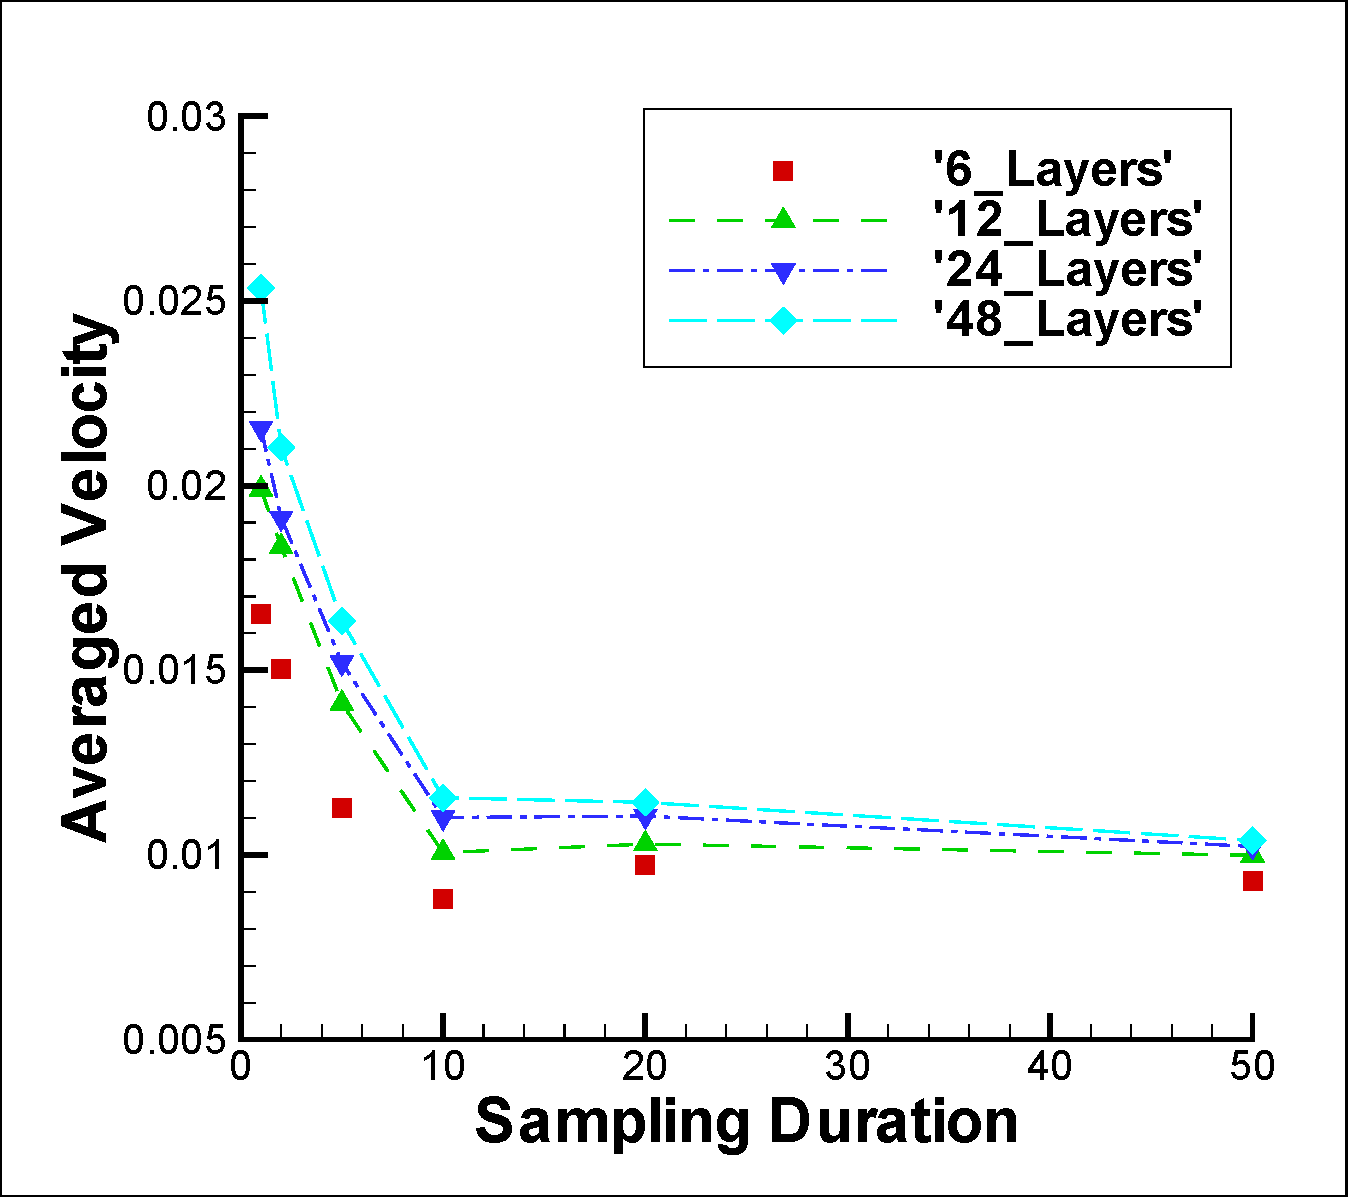
\includegraphics[width=0.4\linewidth]{MD_Regular_Vel0_5e-3.pdf}
\hskip 1cm
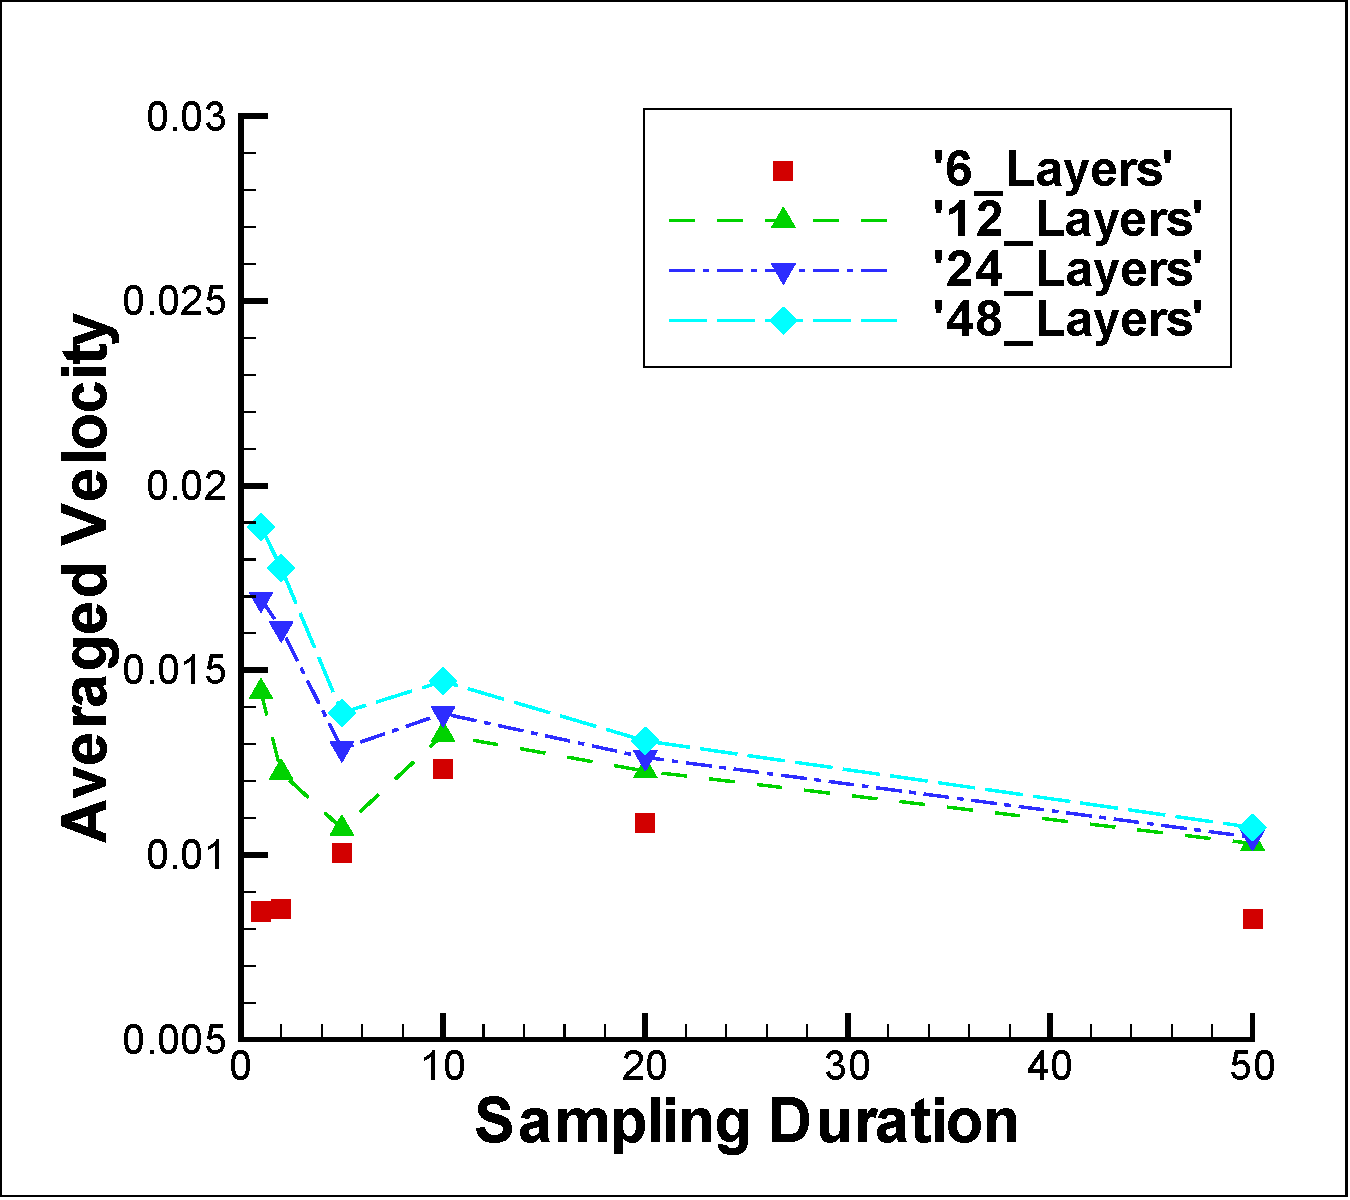
\includegraphics[width=0.4\linewidth]{MD_Regular_Vel0_1e-3.pdf}
\vskip-0.2cm
\caption{\small L2 Norm of Averaged Velocity with Different Layer Sizes and Sampling Duration, at $\Delta{t_{MD}}=5\times{10^{3}}$ (Left) and $\Delta{t_{MD}}=1\times{10^{3}}$ (Right); Solution tends to produce less noise with bigger layer size and smaller MD timescale in short sampling duration. As sampling interval is increased, all solutions converges to the same fluctuation strength, which is 0.01$\sigma/\tau$.}
\label{MD_Regular_Vel0}
\end{figure}



Resulting CFD and MD computational domains are depicted in Fig.~\ref{Couette_Val_Domain}. In CFD mesh, the cell size in Y-direction is 2$\sigma$. Pure MD region is specified to be 10$\sigma$, which was observed to be sufficient to prevent strong fluctuation between fluid particles and wall materials from directly transported to CFD domains by iterative testruns. Two layer boundary zones from particle to continuum domain is placed ahead of pure MD region, from 10 to 14$\sigma$. Continuum to particle boundary is positioned from 18 to 22$\sigma$ and external force region is place at the top of hybrid region, from 24 to 26$\sigma$. MD domain has sufficiently large length in the principal flow direction, to include enough number of particles in the hybrid data average region.

%
\begin{figure}[ht]
\centering
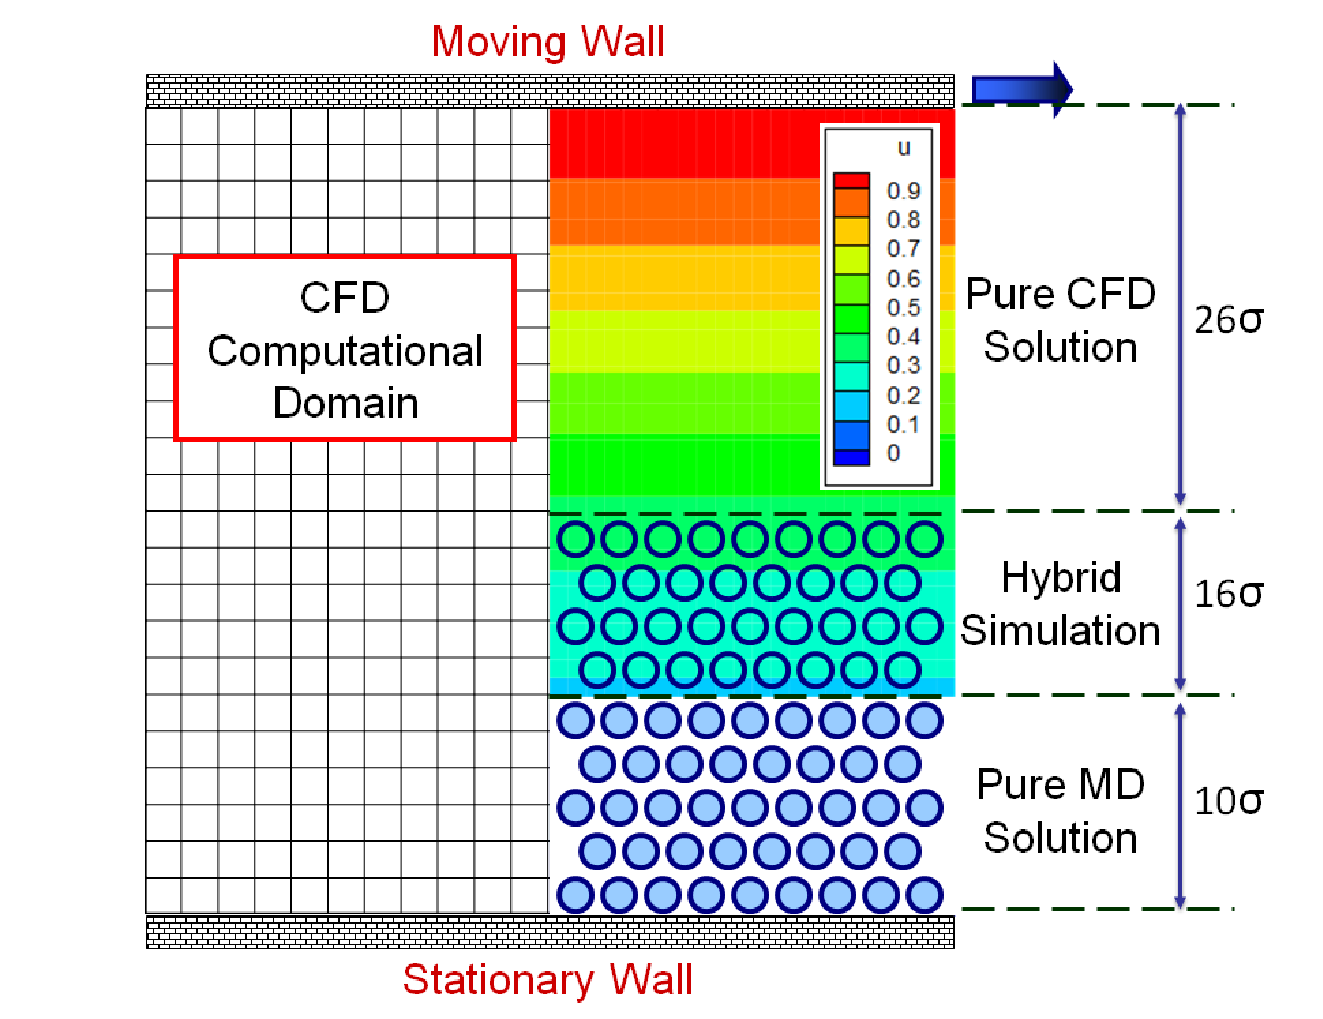
\includegraphics[width=0.6\linewidth]{Couette_Val_Domain.pdf}
\vskip-0.2cm
\caption{\small Computational Domain of Couette Flow Simulation; The height of the fluid domain is 52$\sigma$ ($\approx$177$\AA$). CFD mesh size is 201$\times$27 and CFD cells at the pure MD region are treated as holes. MD domain size is about 210$\sigma$ in the X-direction and around 30$\sigma$ in the Y-direction, including the bottom wall. Periodic boundary condition is applied on the principal flow direction.}
\label{Couette_Val_Domain}
\end{figure}



Unsteady Couette flow profile by CFD, MD and hybrid simulations are presented in Fig.~\ref{Flat_Plate_Sol}. Pure CFD produces identically the same result as analytic solution and MD simulations also describes the same flow physics. In MD simulation, fluctuating pattern is observed during the evolution. This causes the slight variation in hybrid solution, along with the time-lagging in current algorithm. After convergence, the solution follows the same flow pattern as steady profile, which proves that the hybrid approach can accurately analyze the steady flow profile in micro-scaled systems.

%
\begin{figure}[ht]
\centering
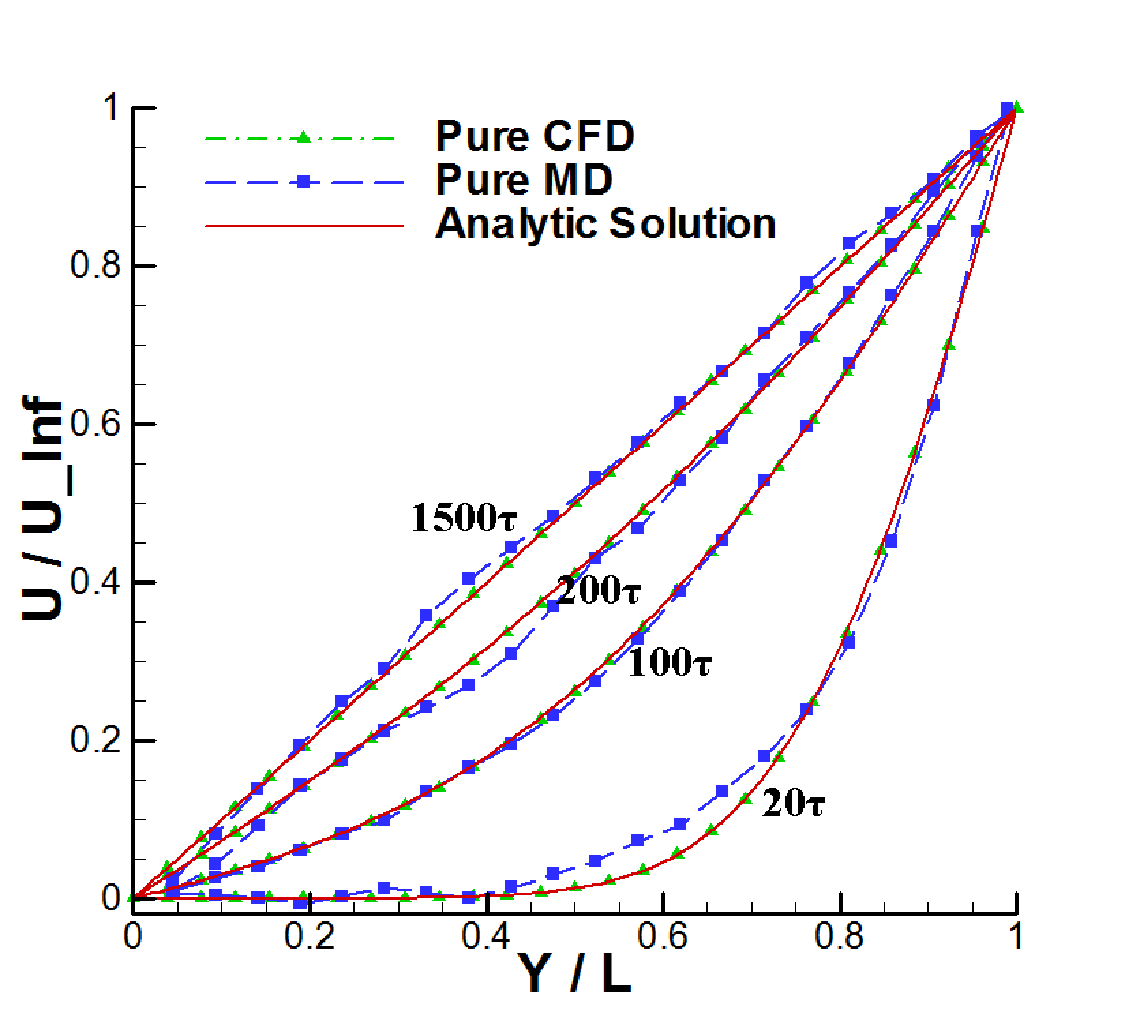
\includegraphics[width=0.4\linewidth]{Flat_Plate_Sol1.pdf}
\hskip 1cm
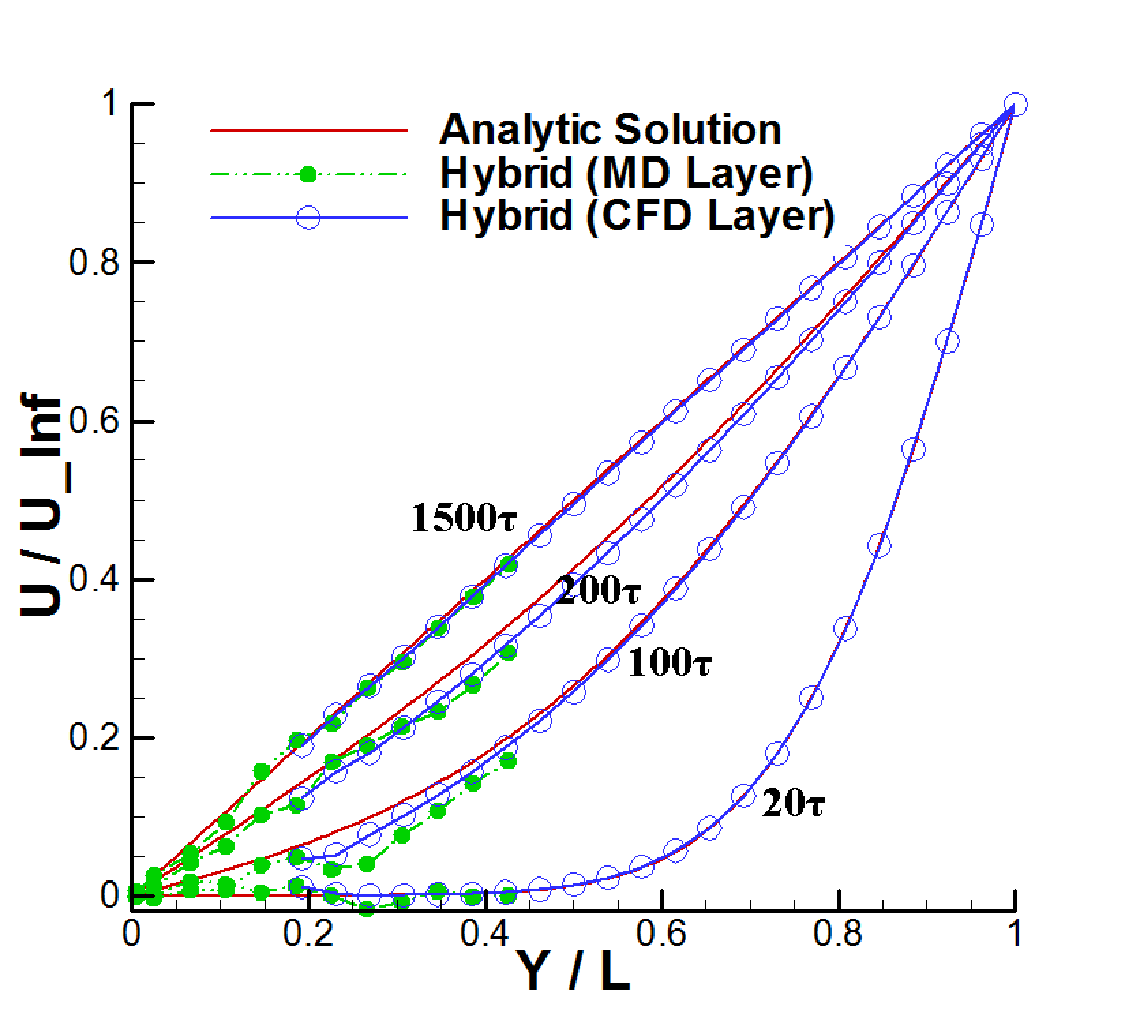
\includegraphics[width=0.4\linewidth]{Flat_Plate_Sol2.pdf}
\vskip-0.2cm
\caption{\small Unsteady Couette Flow Profile; (Left) Pure CFD solution is exactly the same as analytic solution. MD solution shows the same flow pattern as analytic solution, though some fluctuation is observed. This verifies that CFD and MD represents the same flow physics. (Right) The steady result by hybrid approach produces the same numerical result as analytic solution, though the time-lagging in the hybrid boundary is observed during the evolution.}
\label{Flat_Plate_Sol}
\end{figure}



The same domain with coupling condition is applied to solve the Stokes boundary layer problem, which is purely unsteady problem. In this case, the upper wall boundary condition changes from the fixed velocity to oscillatory wall, which is $u_{wall}(t)=({\sigma}/{\tau}){\times}sin(2{\pi}t/T)$. Period $T$ is set 200$\tau$. Velocity in the hybrid region becomes far slower than the Couette flow profile, so the influence of noise from MD side is concerned to be more critical in the current flow simulation.

Figure~\ref{Stokes_Sol} shows the oscillatory velocity profile by pure CFD and hybrid simulations. Unsteady profile in both simulations are globally the same, proving that the current approach can be directly applied to unsteady problems. In detail, fluctuation in MD domain is not so strong in hybrid region. Though minor time-lagging profile is seen from MD solution, this does not change the global flow profile dominantly because the driving force in this simulation is the oscillating velocity from CFD domain.

%
\begin{figure}[ht]
\centering
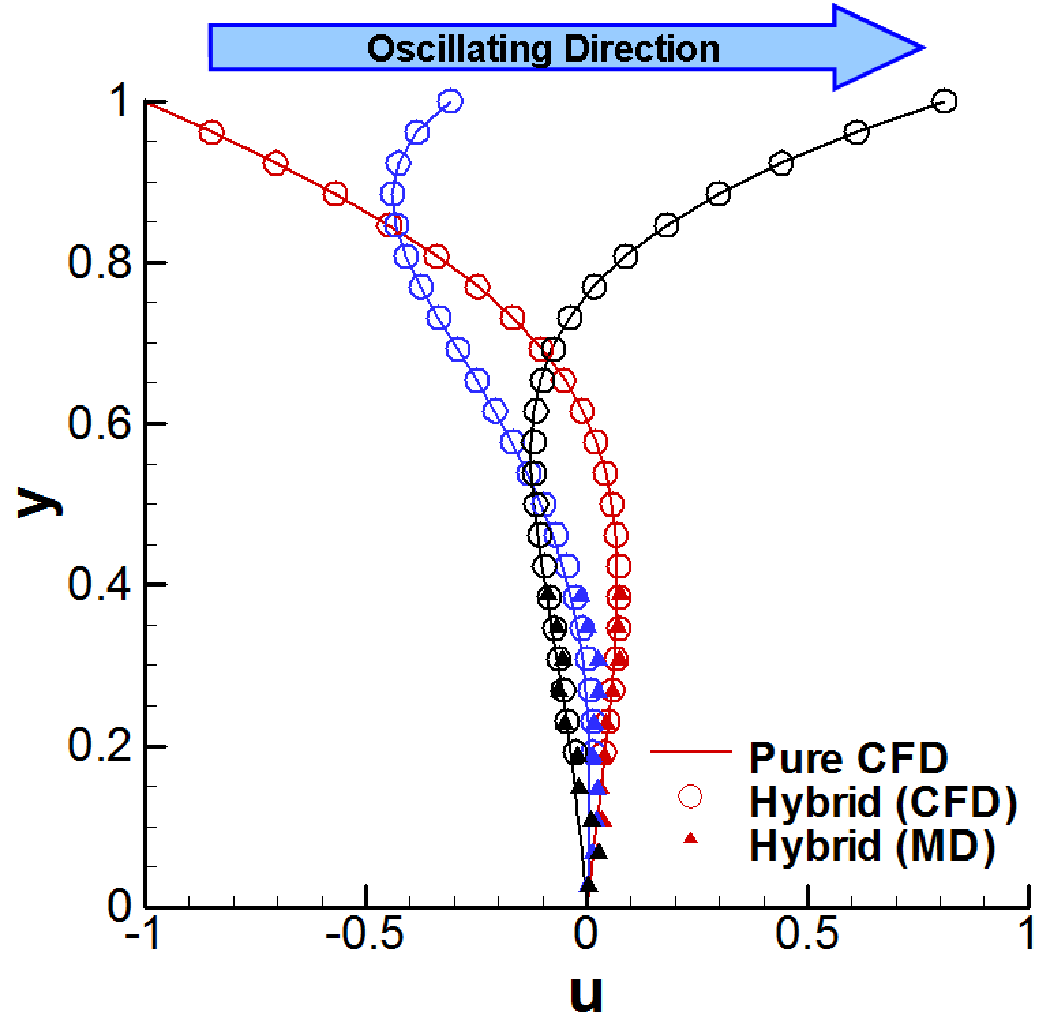
\includegraphics[width=0.4\linewidth]{Stokes_Sol_1.pdf}
\hskip 1cm
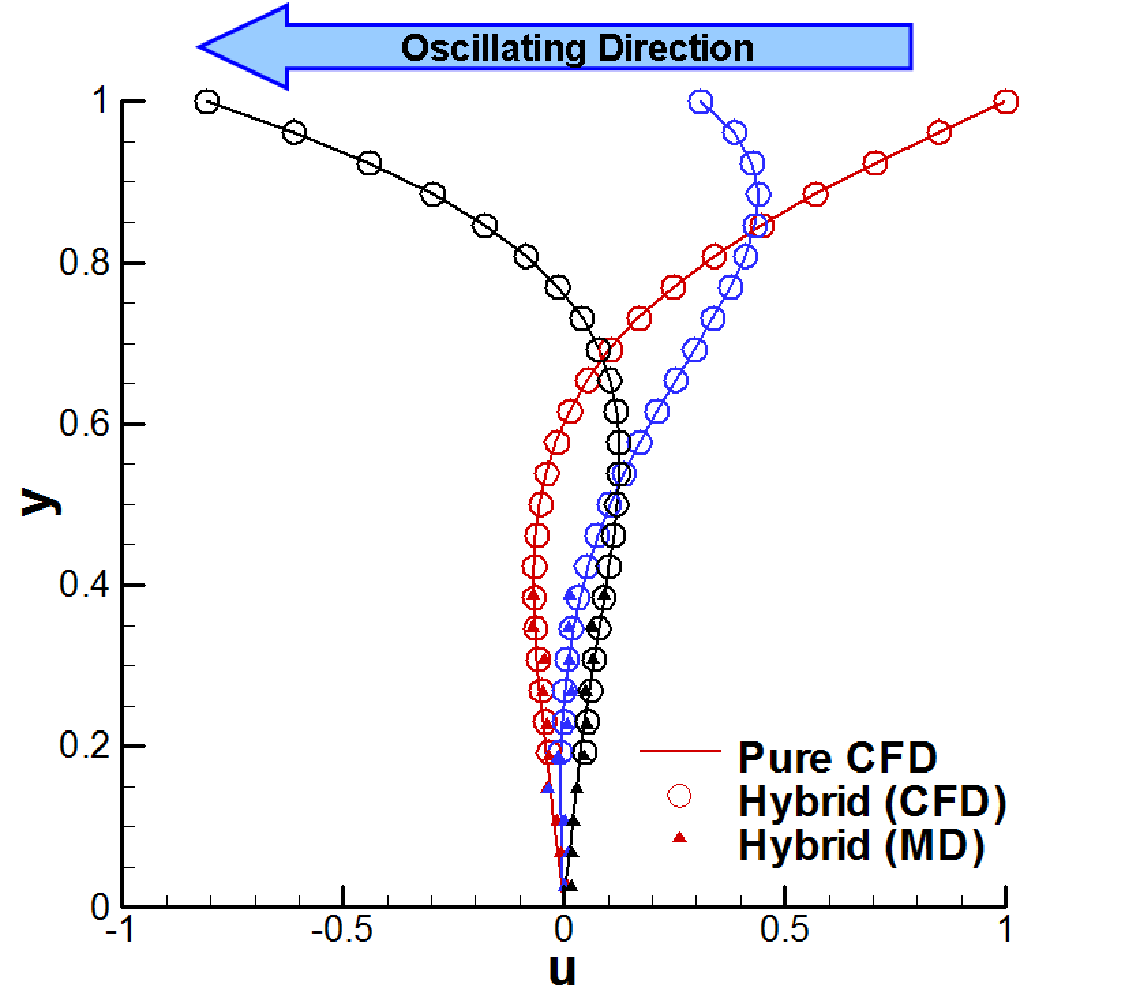
\includegraphics[width=0.4\linewidth]{Stokes_Sol_2.pdf}
\vskip-0.2cm
\caption{\small Unsteady Flow Profile of Stokes Boundary Layer Problem; Solution by pure CFD simulation is denoted by a solid line and solution by hybrid simulation is presented by symbols. Hybrid flow profile globally matches well with CFD solution, though slight time-lagging in the MD side is observed. This evaluates that current hybrid approach can be applied to purely unsteady problem.}
\label{Stokes_Sol}
\end{figure}


\skonote{Additional context after real-scale simulation}


\subsection{Performance Analysis of a Multi-physics Simulation Framework}

\skonote{Queue Wait Time Analysis: Preliminary Test. Waiting Time with Different PX Requests, Wall Time Limit
(Mention that BQP is not perfect, especially measuring inactive waiting time of TWO CONVENTIONAL JOBS)}

The benefit of a BigJob as a way of reducing the waiting time on the local queueing system can be discussed from our preliminary test of the relationship between the requested number of processors and the waiting time.
\newline

\skonote{Already tested waiting time on Ranger: data table and expression will be replaced.}

\begin{table}[t]
  \caption{\small  Effect of various configurations on waiting
    time. The tables show the queue waiting times on Ranger and QueenBee
    with a changing number of processors and different
    requested resource wall-time limits.  Analyzing the
    actual waiting time as a function of the number of processors at different wall-time
    limits, it can be said that better more often than not, the waiting time decrease as the
    requested number of processors increases. The relationship
    between the waiting time and wall-time limit is harder to quantify.
    However, obtained numbers provide a good case study for showing
    the variance of actual queue waiting times.}
\label{table:waitingtime}
\centering
\begin{tabular}
{p{0.4in} || p{0.4in} p{0.4in} p{0.4in} p{0.4in} p{0.4in}}
\multicolumn{6}{c}{\phantom{\tiny 100}}\\
\hline
%\midrule
 \multirow{3}{0.4in}{Number of processors}&
 \multicolumn{5}{c}{Requested wall-time at 92$\pm$6\% load (Ranger)}
\\
\cline{2-6}
%\cmidrule{2-6}
 & \nyc 2hr
 & \nyc 3hr
 & \nyc 4hr
 & \nyc 6hr
% & \nyc 6hr
& \multicolumn{1}{c}{12hr}
%  &1hr &2hr &4hr &6hr &12hr
\\
\cline{2-6}
%\cmidrule{2-6}
 &\multicolumn{5}{c}{Waiting time on the queue [sec]}
\\
\cline{1-1}
%\cmidrule{1-1}
\nyc 16
 & \nyc 9989 & \nyc 15984 & \nyc 39151 & \nyc 65 & \multicolumn{1}{c}{66}
\\
\nyc 32
 & \nyc 15371 & \nyc	4106 & \nyc 11376 & \nyc 54 & \multicolumn{1}{c}{55}
 \\
\nyc 48
  & \nyc 13264 & 4392 \nyc  & \nyc 37780 &\nyc 43 & \multicolumn{1}{c}{44}
\\
\nyc 64
 & \nyc 9944 &	\nyc 1975	 & \nyc 39855 & \nyc 31 & \multicolumn{1}{c}{32}
\\
\hline
%\midrule


\multicolumn{6}{c}{\phantom{100}}\\
\hline
%\midrule
 \multirow{3}{0.4in}{Number of processors}&
 \multicolumn{5}{c}{Requested wall-time at 95$\pm$4\% load (Queenbee)}
\\
\cline{2-6}
%\cmidrule{2-6}
 &\nyc 2hr
 &\nyc 3hr
 &\nyc 4hr
 &\nyc 6hr
 &\multicolumn{1}{c}{12hr}
\\
\cline{2-6}
%\cmidrule{2-6}
 &\multicolumn{5}{c}{Waiting time on the queue [sec]}
\\
\cline{1-1}
%\cmidrule{1-1}
\nyc 16
 & \nyc 14339 & \nyc 3578  & \nyc 39113 & \nyc 6 & \multicolumn{1}{c}{940}
\\
\nyc 32
 & \nyc 14312 & \nyc 3550 & \nyc 39238 & \nyc 5 &\multicolumn{1}{c}{6344}
 \\
\nyc 48
 & \nyc 21555 & \nyc 3517 & \nyc 39207 & \nyc 4 & \multicolumn{1}{c}{6353}
\\
\nyc 64
 & \nyc 21541 & \nyc 3489 & \nyc 39179 & \nyc 3 & \multicolumn{1}{c}{6329}
\\
\hline
%\midrule
\end{tabular}
\vspace{-1em}
\end{table}

We designed experiments to determine if running larger and/or longer simulations effects the actual waiting time on the queue. We performed our experiments on machines spanning two orders of magnitude in size (and peak performance)-- from approximately 500 px to 65000 px, and for a range of load-factors.  We submitted jobs of different sizes, requiring different wall-time limits. Each time we submitted a job, we gathered the load-factor and the actual waiting time on the queue. Many factors effect the waiting times, arguably the most important of them are the load-factor at the instant of submission, requested wall-time limit and also the number of processors requested. Two other factors that effect this are the backfilling that occurs when some other unrelated job finishes and the changes in the priority of the test job when a particular higher priority job joins the queue; however, unlike the first three factors, the last two are somewhat random and it is difficult to systematically account for them. Also, the internal queueing policy of supercomputing centers may effect the waiting time on the queue based on their queueing priority including credential, fairshare, resource and service priority.  As can be seen from Table~\ref{table:waitingtime}, the waiting time tends to decrease as the number of processors requested in a job increases.

Results for machines with more than 5000 px, Ranger and Queenbee are presented in Table~\ref{table:waitingtime}, and as can be seen, jobs with larger processor counts have typically lower wait times. The observation holds true for a range of values of requested wall-times over a range of ``high'' load-factors.

It is however, difficult to discern a relationship between waiting time with the requested wall-time limit of jobs; from experience there is greater variation in backfilling probability with varying wall-time requests.  However, as we are able to establish that a single large job on average has to wait less at the queue than a smaller job does, most definitely the maximum wait time of two small jobs will be even greater. In other words the sum total of the waiting time (of the first-to-run job) and the inactive time (defined as the difference between the waiting time of the two jobs) will be larger than the wait time of a single large job.
\newline


\skonote{Queue Wait Time Analysis: Waiting time of a BigJob and two conventional jobs. Emphasize the inactive time as well - it makes the conventional job submission to have longer wall time limit and it will even reduce the possibility of getting the backfilling capability. Include Table 2 here.}

A BigJob submission shows the saving of waiting time on the queue, not only the bigger job size has the higher priority in the queueing system but also one BigJob submission eliminates the inactive idling time of first allocated job in conventional job submission.
\newline

\skonote{More test conducted on Ranger. Table needs replacement.}

Controlling runtime in these two scenarios, i.e., we take a BigJob of size 2X and 2 conventional jobs of size X each, we compare the waiting time of a 64 px BigJob (with wall-clock limits of 2, 3, and 4hrs) which is smaller than the wait for a 32 px conventional job for the same values of wall-clock limits. As the individual simulations are assigned the same number of processors, the runtime performance will be similar in the two scenarios, and thus the total time-to-solution will determined by the wait-times on queues -- which we show statistically to be lower for the larger BigJob submission mode.

\begin{table}[t]
  \caption{\small  Waiting and inactive time for conventional job
    submissions, and a single BigJob submission. All measured times are in seconds and expressed as 'mean$\pm$SD'. In both cases,
    conventional job is submitted to use 2$\times$32 px and a
    BigJob requests 64 px on small and less crowded LONI clusters. Conventional job submission mode showed faster
    time-to-start (i.e., the sum of waiting time and inactive mode) on
    small problem size with 6 hr of wall-time limit, while a BigJob
    gets allocated faster with longer wall-time limit. Conventional job
    submission showed 3 failures during the test due to the timeover of
    wall-time limit in the first-started job.}
\label{table:BJwaiting}
\centering
\begin{tabular} {p{0.55in} || p{0.7in} p{0.7in} p{0.7in}}
\multicolumn{4}{c}{\phantom{\tiny 100}}\\
\hline
 \multirow{2}{0.55in}{}&
 \multicolumn{3}{c}{Small simulation with 6 hr wall-time limit}
\\
\cline{2-4}
 & \nyc Waiting time
 & \nyc Inactive mode
 & \multicolumn {1}{c}{Failed runs}
\\
 \hline
   \nyc Conventional & \nyc 12318$\pm$15649 & \nyc 7407$\pm$11375 & \multicolumn {1}{c}{2} \\
  \nyc 1 BigJob & \nyc 29452$\pm$31946 & \nyc 0 & \multicolumn {1}{c}{0} \\
 \hline

\multicolumn{4}{c}{\phantom{100}}\\
\hline
 \multirow{2}{0.55in}{}&
 \multicolumn{3}{c}{Large simulation with 24 hr wall-time limit}
\\
\cline{2-4}
 & \nyc Waiting time
 & \nyc Inactive mode
 & \multicolumn {1}{c}{Failed runs}
\\
\hline
 \nyc Conventional & \nyc 83102$\pm$77134 & \nyc 47488$\pm$55647 & \multicolumn{1}{c}{1}
\\
 \nyc 1 BigJob & \nyc 76645$\pm$55474 & \nyc 0 & \multicolumn{1}{c}{0}
\\
\hline

\end{tabular}
\vspace{-1em}
\end{table}


Results for smaller systems ($\approx$ 500 px) are presented in a different fashion in Table~\ref{table:BJwaiting}. In addition to the fact that a 64 px BigJob is now around 16\% of the machine resources, the load-factors of the smaller machines fluctuated much more than those of the larger machines. Consequently the data obtained for smaller resources is far more noisier and than the ``clean'' data for the larger machines -- Ranger and QueenBee. As can be seen from Table~\ref{table:BJwaiting} although the waiting time for the first-to-start job was smaller in the conventional job submission mode than the BigJob (S1), the second job (convention job) had a large subsequent wait time; thus for conventional job submission mode there is a non-negligible inactive mode (defined as the time difference between queue wait times between the two simulations). There is no inactive mode for BigJob submission as by defintion both simulations begin concurrently. Interestingly, the situation is somewhat worse for the conventional job submission; although the average wait time is lower than the BigJob, there exist 2 (out of 6) cases (for 6hr wall-clock limit), when the wait time of the second job is greater than the wall-clock limit for the first-to-start job. In other words, the second job fails to start in the duration that the first-to-start job is in active/run mode, but can't do anything useful as the second job is still waiting on the queue. This is typically alleviated with co-allocation of resources; however the number of production grid infrastucture that provide co-allocation (and co-scheduling) as a production service is very limited. This leads us to the heart of the advantage of the BigJob submission mode: circumventing the requirements of co-scheduling by providing an application level solution that preserves performance and guarantees non-failure due to large-fluctuations (see data for 24hr wall-time limit) in queue waiting times.



\skonote{Runtime Analysis: Comparison of LB with conventional simulation time: different system size (with different ratio between CFD and MD), different number of simulation loop and different interval of simulation loop. Table 3 with 2 graphs - change of CPU allocation to each subjob with iteration time in 2 simulation cases. Mention the problem size and setting a little more detail.}

Runtimes of the coupled simulation with a single BigJob is given on Table~\ref{table:oneBJ_Test}. For both small and large simulations, a default BigJob task takes about 1 percent longer than the conventional test. This is reasonable because a default BigJob has the same processor distribution between sub-jobs as the conventional job, while BigJob has the minor overhead of sub-jobs' status monitoring and communication with advert server. In cases of load-balanced BigJob simulations, there is a significant reduction in the runtime compared to successful conventional jobs -- 13\% and greater. For larger problem set, a load-balanced BigJob simulation relatively shows higher standard deviation (SD) due to the unexpected instability of a computing resource during one experiment, to be discussed in detail below.

\begin{table}[t]
%\setlength{\tabcolsep}{1pt}
%\begin{table}[!ht]
%\begin{center}
  \caption{\small Results of runtime for S1, $S1_{LB}$ and
    conventional submission. All measured times are in seconds and expressed as 'mean$\pm$SD'. 6 distinct experiments were accomplished
    for each simulation, all with 64 px. In both cases, S1 shows about 1\% overhead
    due to the communication with advert server. On the other hand,
    $S1_{LB}$ tests show about 13\% runtime save compared to
    conventional submission.}
\label{table:oneBJ_Test}
\centering
\begin{tabular} {p{0.5in} || p{0.7in} p{0.7in} p{0.7in}}
  \multicolumn{4}{c}{\phantom{\tiny 100}}\\
  \hline
  & \nyc Conventional
  & \nyc S1
  & \multicolumn{1}{c}{$S1_{LB}$}
  \\
  \hline
  \nyc Small sim. & \nyc 757$\pm$1.89 & \nyc 764$\pm$1.41 & \multicolumn{1}{c}{661$\pm$4.41} \\
  \nyc Large sim. & \nyc 39595$\pm$119.2 & \nyc 39906$\pm$206.3 & \multicolumn{1}{c}{34350$\pm$1302.7} \\
  \hline
%\midrule
\end{tabular}
\vspace{-1em}
\end{table}

The validity of a load balancing function can be discussed by the change of processor distribution between subtasks throughout the simulation. For the result of a small simulation in Fig.~\ref{Fig:LBSmall}, both CFD and MD subtasks are assigned with 32 px initially. After two simulation loops, a load balancer converges to the processor distribution of 12 to 52 px between CFD and MD respectively; this processor distribution remains the same until the simulation completes. Runtime per loop is reduced from 153 sec for the first loop to 107 sec after the convergence. Total computation time is 596.19 sec, which is different from 663 sec counted from BigJob application manager. This time difference implies that the BigJob application manager spends about 13 sec per stage in executing its internal commands including the run of a load balancing function and sub-job re-launch.


%%%%% FIGURE %%%%%
\begin{figure}
%\vspace{-1em}
\centering
%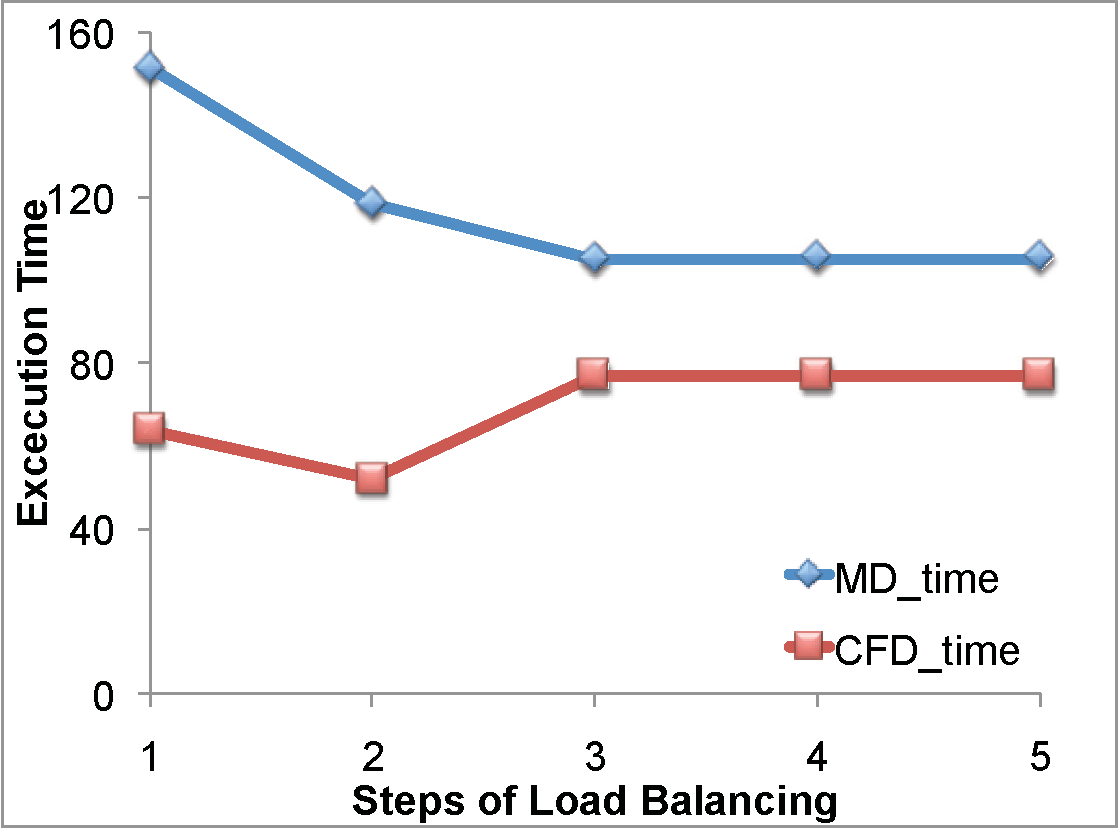
\includegraphics[scale=0.3]{fig6_1.pdf}
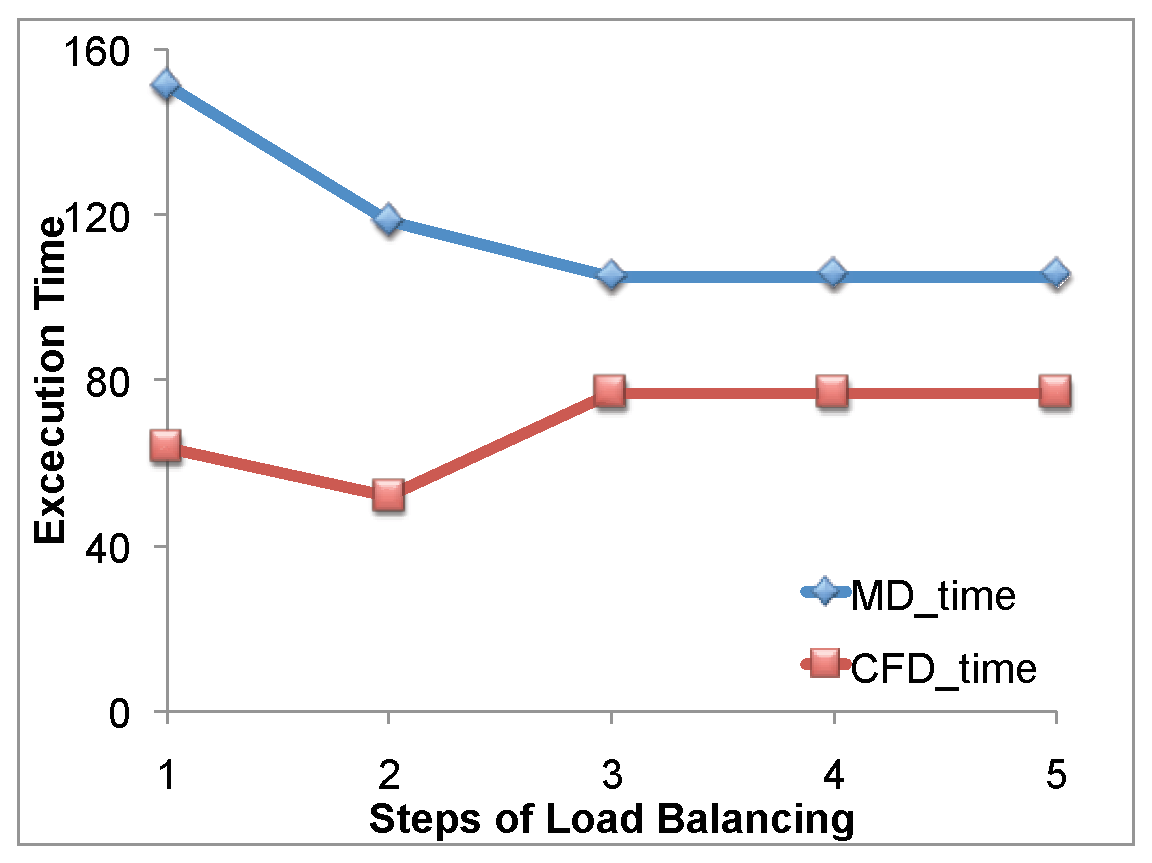
\includegraphics[scale=0.3]{fig6_1.eps}
\linebreak
%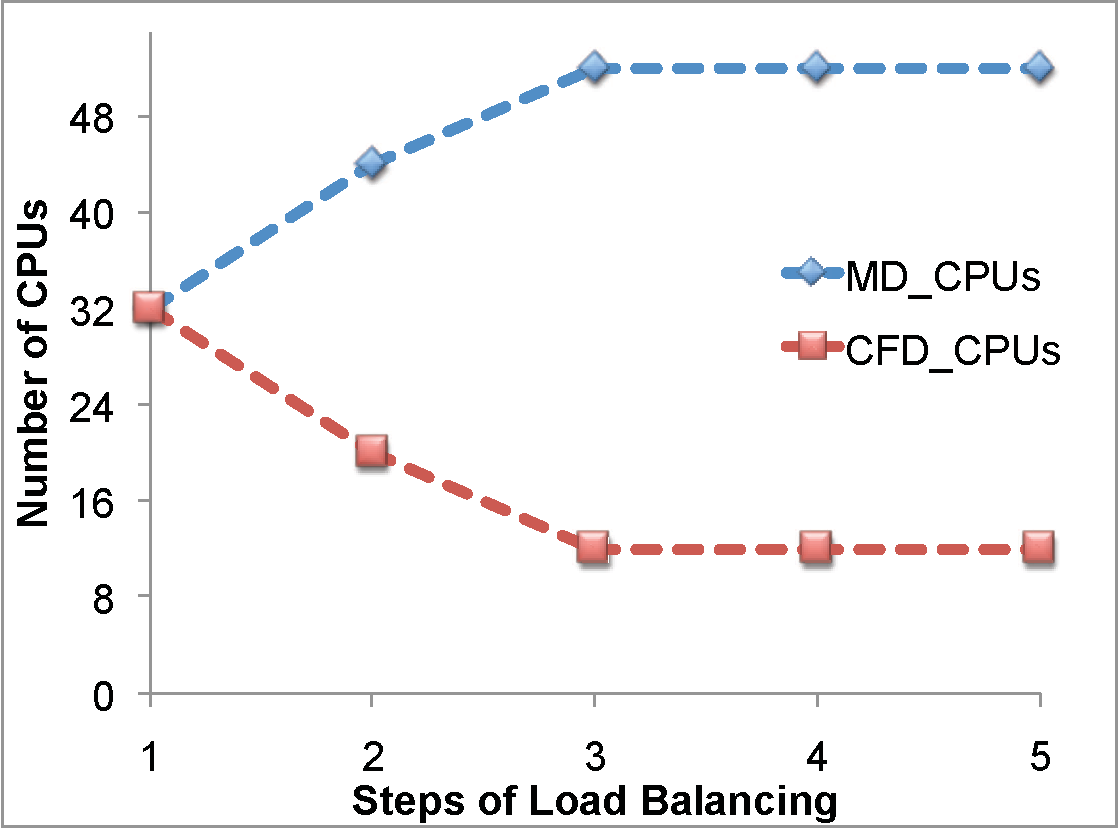
\includegraphics[scale=0.3]{fig6_2.pdf}
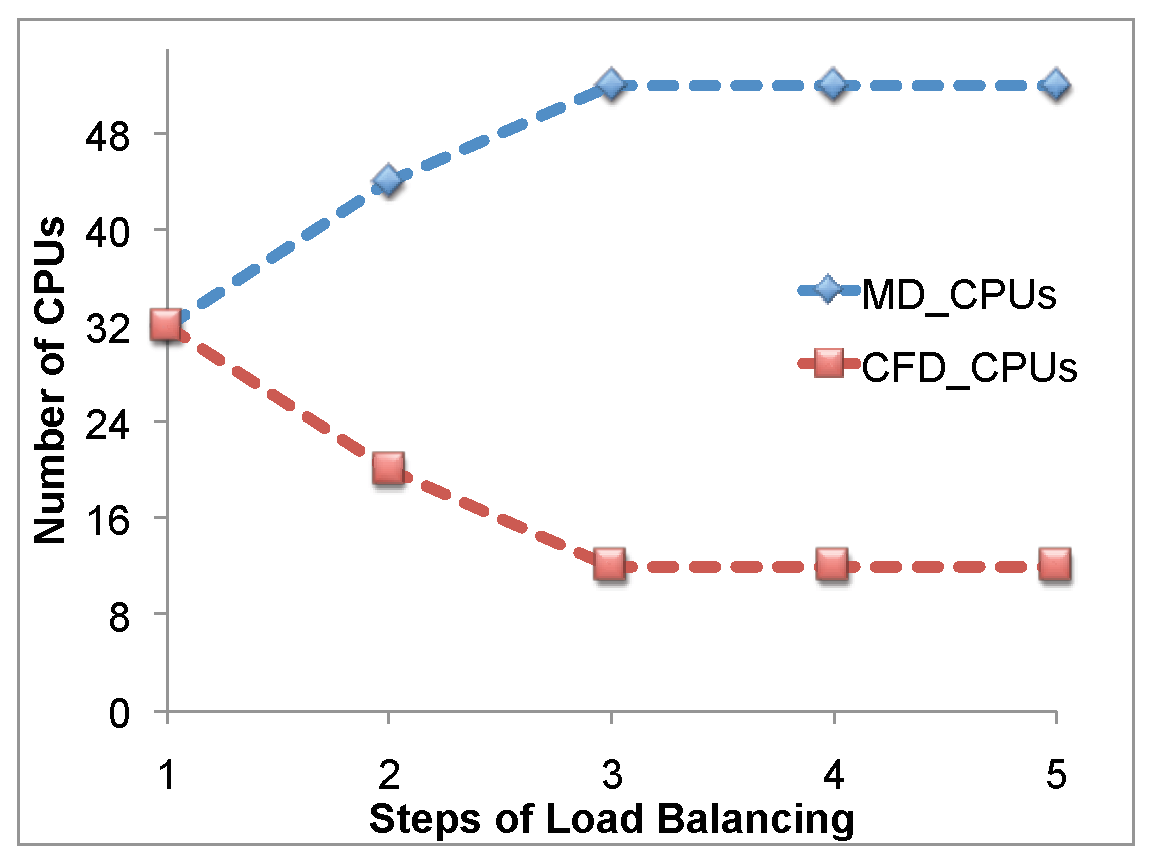
\includegraphics[scale=0.3]{fig6_2.eps}
\caption{\small Change of processor distribution between CFD and MD
  jobs and resultant computation time in the small simulation. A load
  balancer starts from the same number of processors assigned to both
  sub-jobs and detects 20 to 44 px between each sub-job as the optimal
  solution. The poor scalability of CFD job makes the load balancer to
  search for the optimal condition once again and the processor
  assignment finally reaches to a steady solution of 12 to 52 between
  two sub-jobs. Computation time for every simulation loop reduces
  from 153 sec to 107 sec after the balancing.}
\label{Fig:LBSmall}
\vspace{-1em}
\end{figure}
%%%%% FIGURE %%%%%


The result of computation time evolution for a large simulation is seen in Fig.~\ref{Fig:LBLarge}. For most experiments, which is given in the left side of Fig.~\ref{Fig:LBLarge}, a load balancer directly goes to a converged solution of processor distribution, which is 24 to 40 between CFD and MD jobs. On the other, in one experiment, computing nodes assigned to MD simulation seem to have temporarily experienced the internal overhead as shown from the right side of Fig.~\ref{Fig:LBLarge}. This overhead temporarily increased MD computation time a lot and a load balancer shows the fluctuating pattern of processor distribution in response to this temporary instability. A load balancer goes to a different steady solution after the system settled down, which is the processor distribution of 20 to 44 between two sub-jobs. Compared to the steady solution in stable cases, computation time for one simulation loop increases in this processor distribution increases from 1320 sec to 1380 sec.

Plots on the right side of Fig.~\ref{Fig:LBLarge} show a non-monotonically changing resource assignment by the LB, and thus demonstrating how the load balancer can be self-correcting and adapt to changing performance; after increasing the number of processors assigned to the MD, the load-balancer unassigns the additional processors.


% %%%%% FIGURE %%%%%
\begin{figure}
%\vspace{-1em}
\centering
%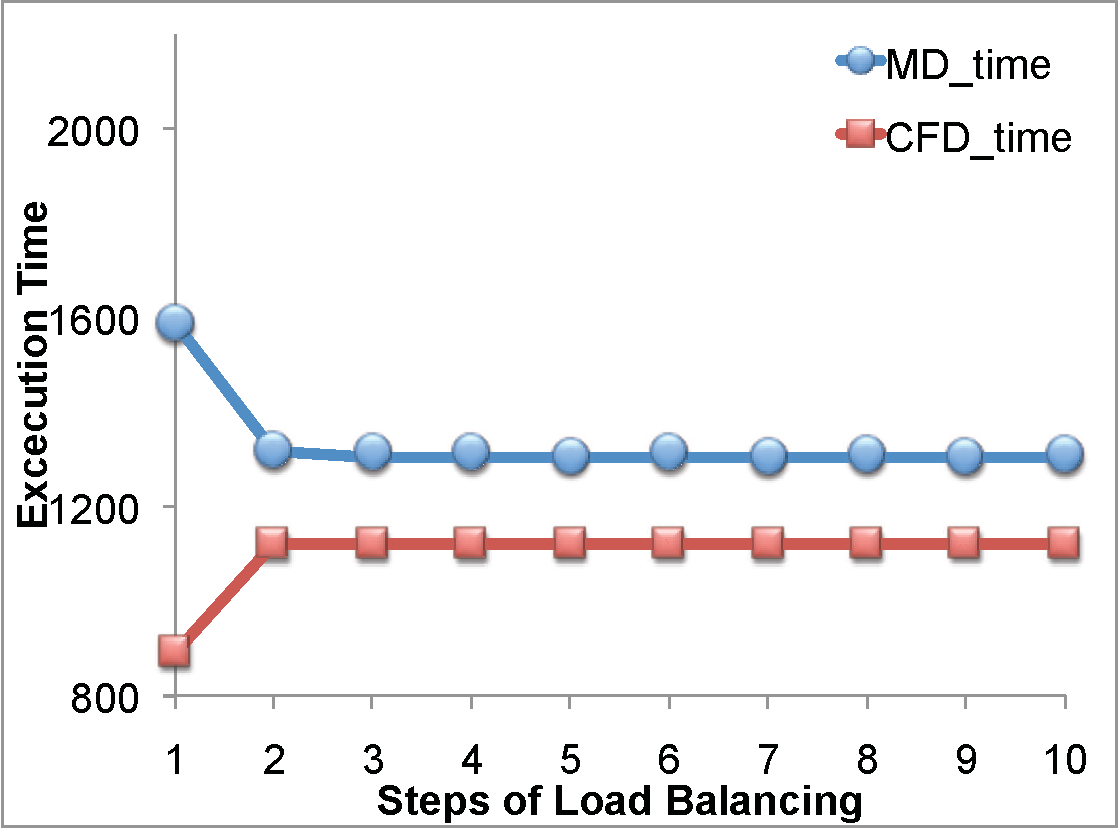
\includegraphics[scale=0.21]{fig7_11.pdf}
\includegraphics[scale=0.21]{fig7_11.eps}
%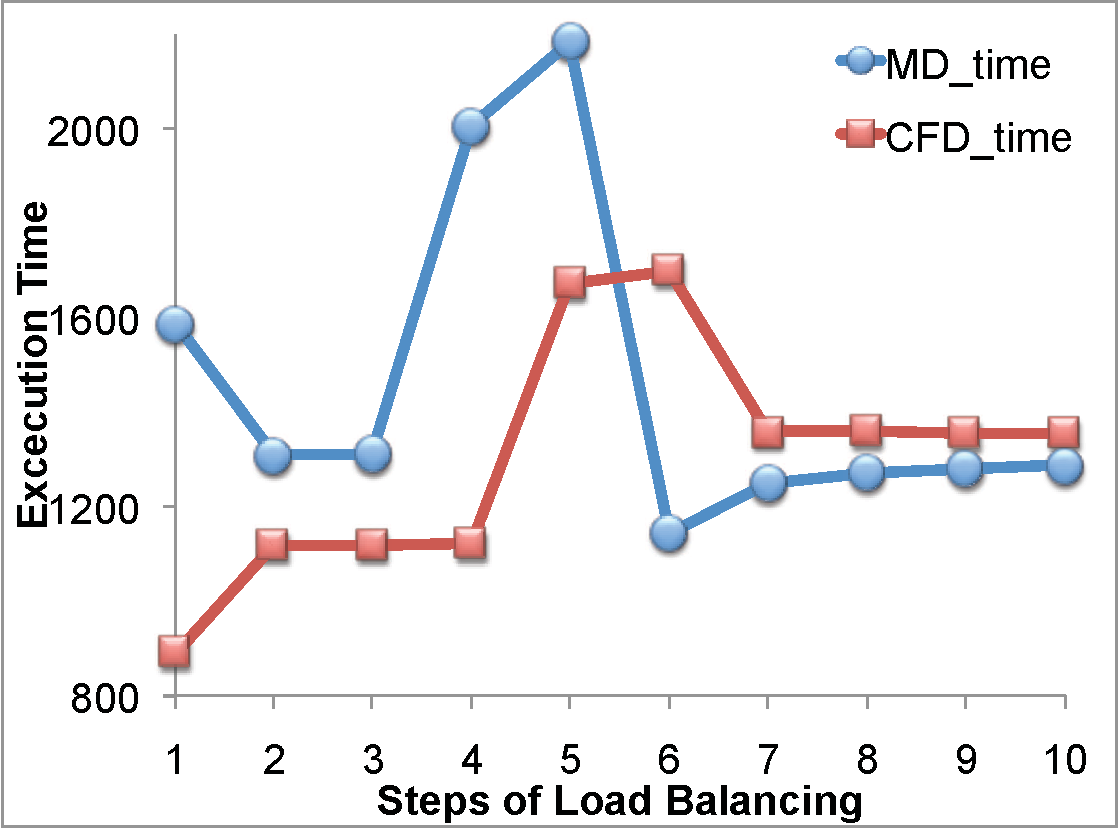
\includegraphics[scale=0.21]{fig7_21.pdf}
\includegraphics[scale=0.21]{fig7_21.eps}
\linebreak
%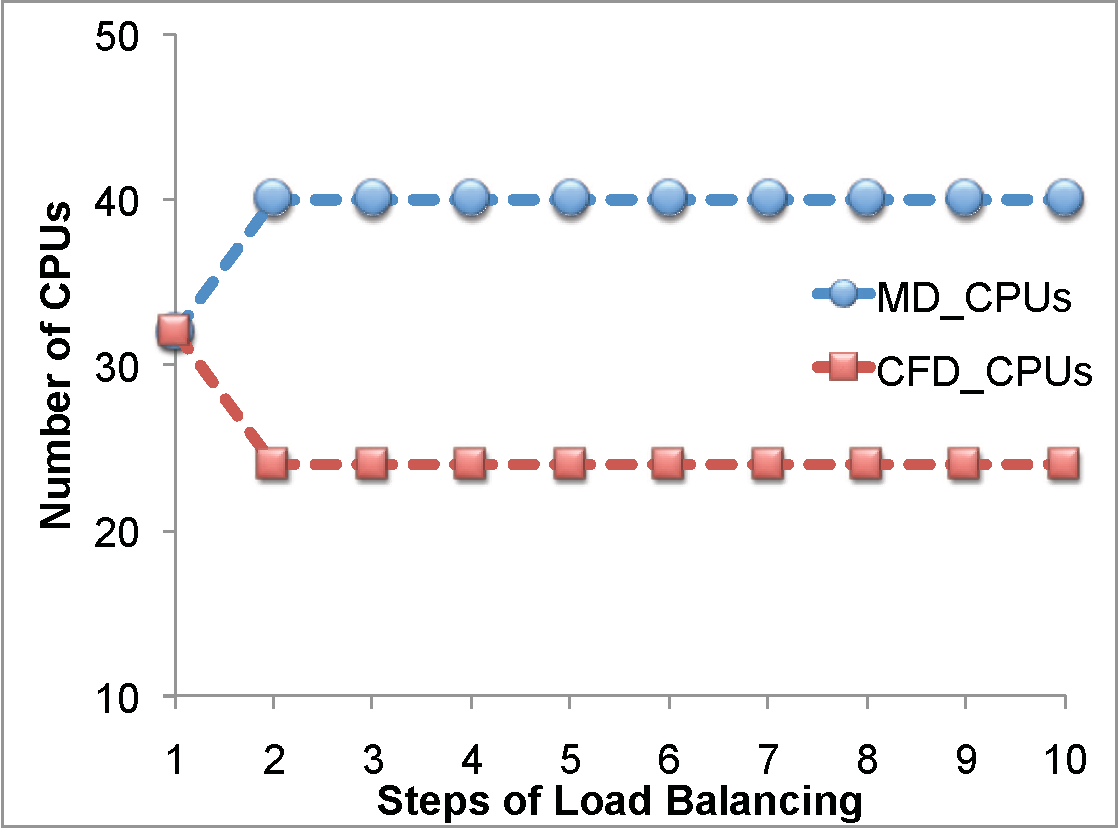
\includegraphics[scale=0.21]{fig7_12.pdf}
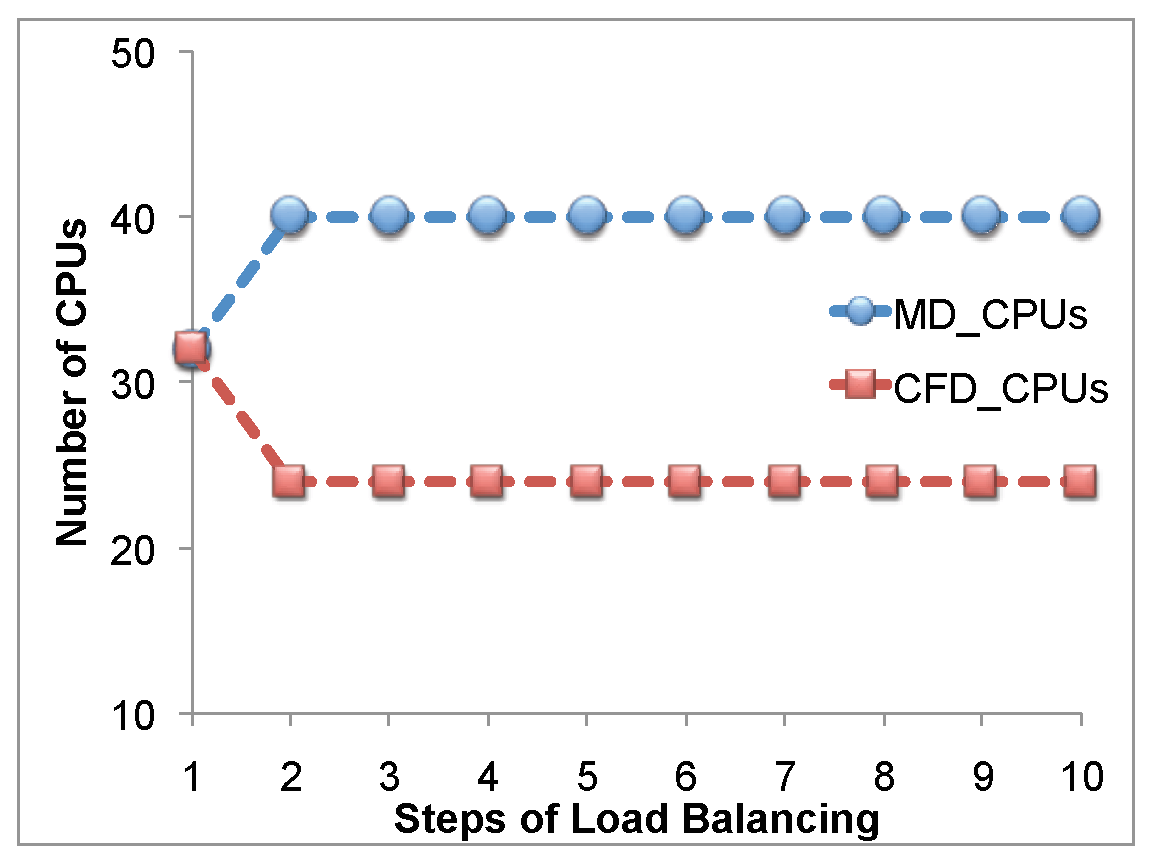
\includegraphics[scale=0.21]{fig7_12.eps}
%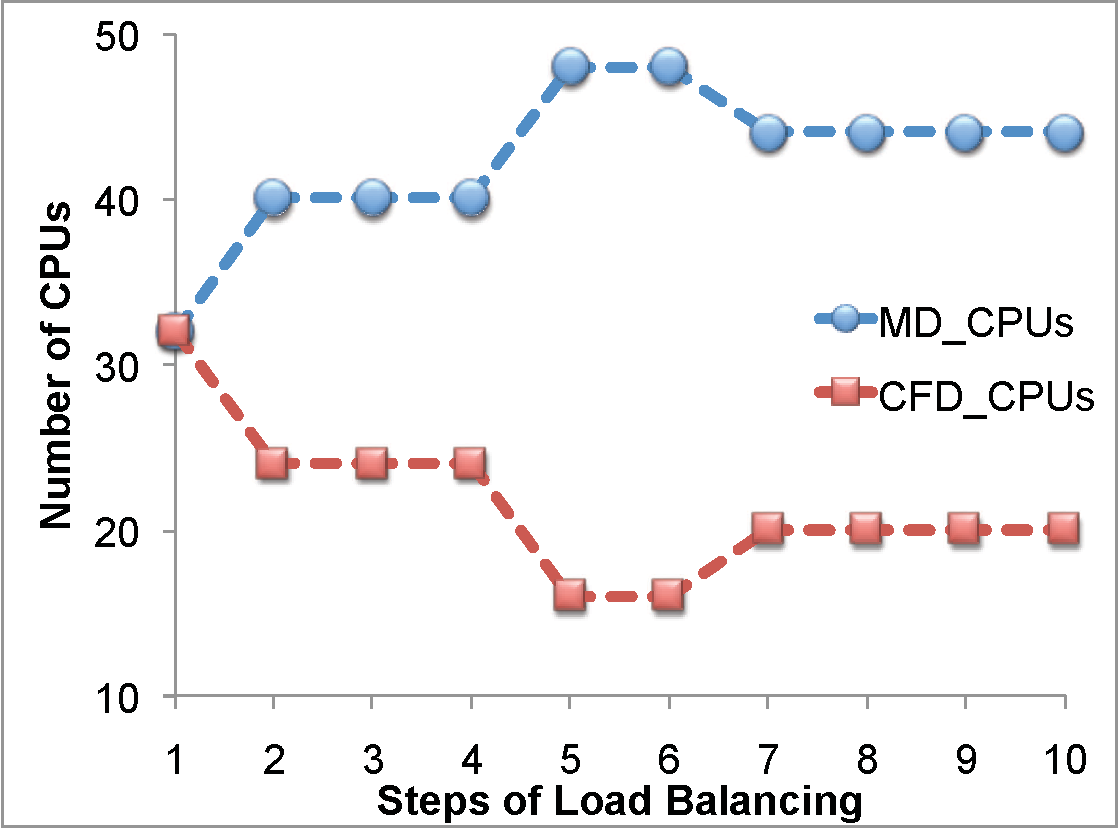
\includegraphics[scale=0.21]{fig7_22.pdf}
\includegraphics[scale=0.21]{fig7_22.eps}
\caption{\small (Left Column) Change of processor distribution between
  CFD and MD jobs and resultant computation time in the large
  simulation. A load balancer directly finds the processor
  distribution of 24 to 40 between CFD and MD jobs and remains the
  steady state until it completes after 25 simulation loops. Initial
  computation time of 1605 sec reduces to 1320 sec after the
  convergence. (Right Column) Plots showing non-monotonic resource
  assignment by the LB, and thus demonstrating how the load balancer
  can be self-correcting and adapt to changing performance; after
  increasing the number of processors assigned to the MD, the
  load-balancer unassigns the additional processors.}
\label{Fig:LBLarge}
\vspace{-1em}
\end{figure}
%%%%% FIGURE %%%%%



%-------------------------------------------------------------------------
\section{Next Step: Further Refinement}


%-------------------------------------------------------------------------
\section{Conclusions}



\section*{Acknowledgment}
This work is part of the Cybertools (http://cybertools .loni.org)
project and primarily funded by NSF/LEQSF (2007-10)-CyberRII-01.
Important funding for SAGA has been provided by the UK EPSRC grant
number GR/D0766171/1 (via OMII-UK). This work has also been made
possible thanks to computer resources provided by LONI. We thank Andre
Luckow for initial work on BigJob, Lukasz Lacinski for help with SAGA
deployment (via HPCOPS NSF-OCI 0710874) and Joao Abecasis for his work
on the SAGA Condor adaptors.

%-------------------------------------------------------------------------
\nocite{ex1,ex2}
\bibliographystyle{IEEEtran}
\bibliography{saga_tg08}


\end{document} 